\section{Example Computations}

To get feel for the model, let's look at some example computations.

\paragraph*{Addition}
Let's try to implement addition in the Colored Graph model.
We represent a number $n$ by a chain of $n+1$ nodes connected to each other with blue edges.
The reason that we use $n+1$ and not $n$ to be able to represent 0 with a single node.
Then to add two number, we will connect the two chains together with a red edge to a long chain.
So the input to our program to add 3 and 5 will be the following graph.

\begin{center}
    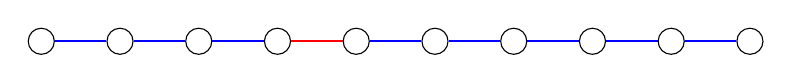
\begin{tikzpicture}
        \node[circle,draw] (A) at (1,0) {};
        \node[circle,draw] (B) at (2,0) {};
        \node[circle,draw] (C) at (3,0) {};
        \node[circle,draw] (D) at (4,0) {};

        \node[circle,draw] (E) at (5,0) {};
        \node[circle,draw] (F) at (6,0) {};
        \node[circle,draw] (G) at (7,0) {};
        \node[circle,draw] (H) at (8,0) {};
        \node[circle,draw] (I) at (9,0) {};
        \node[circle,draw] (J) at (10,0) {};
        
        \draw[blue, thick] (A) -- (B);
        \draw[blue, thick] (B) -- (C);
        \draw[blue, thick] (C) -- (D);
        \draw[red, thick] (D) -- (E);
        \draw[blue, thick] (E) -- (F);
        \draw[blue, thick] (F) -- (G);
        \draw[blue, thick] (G) -- (H);
        \draw[blue, thick] (H) -- (I);
        \draw[blue, thick] (I) -- (J);
    \end{tikzpicture}
\end{center}

To add these two numbers we simply need the following rule.

\begin{center}
    \begin{tikzpicture}
    \begin{scope}[xshift=-2cm]
        \node[circle,draw] (A) at (-1, 0) {};
        \node[circle,draw,fill] (B) at (0,0) {};
        \node[circle,draw] (C) at (1,0) {};
        
        \draw[blue, thick] (A) -- (B);
        \draw[red, thick] (B) -- (C);
    \end{scope}

    \draw [line width=1pt, double distance=3pt, arrows = {-Latex[length=0pt 3 0]}] (-0.5,0) -- (0.5,0);
    
    \begin{scope}[xshift=2cm]
        \node[circle,draw] (A) at (-1, 0) {};
        \node[circle,draw] (C) at (1,0) {};
        
        \draw[blue, thick] (A) -- (C);
    \end{scope}
    \end{tikzpicture}
\end{center}

This rule can be applied to either of the nodes connected to the red edge and in one step will produce the correct restult.

\begin{center}
    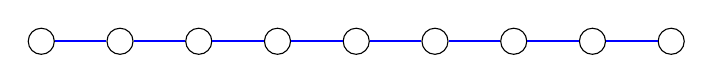
\begin{tikzpicture}
        \node[circle,draw] (A) at (1,0) {};
        \node[circle,draw] (B) at (2,0) {};
        \node[circle,draw] (C) at (3,0) {};
        \node[circle,draw] (D) at (4,0) {};

        \node[circle,draw] (E) at (5,0) {};
        \node[circle,draw] (F) at (6,0) {};
        \node[circle,draw] (G) at (7,0) {};
        \node[circle,draw] (H) at (8,0) {};
        \node[circle,draw] (I) at (9,0) {};
        
        \draw[blue, thick] (A) -- (B);
        \draw[blue, thick] (B) -- (C);
        \draw[blue, thick] (C) -- (D);
        \draw[blue, thick] (D) -- (E);
        \draw[blue, thick] (E) -- (F);
        \draw[blue, thick] (F) -- (G);
        \draw[blue, thick] (G) -- (H);
        \draw[blue, thick] (H) -- (I);
    \end{tikzpicture}
\end{center}

To deal with the special case of $0 + 0$, for which this rule does not work we will add the following Delete Rule that just removes a node connected to exactly one red edge and has an empty rewiring.

\begin{center}
    \begin{tikzpicture}
    \begin{scope}[xshift=-2cm]
        \node[circle,draw,fill] (B) at (0,0) {};
        \node[circle,draw] (C) at (1,0) {};
        
        \draw[red, thick] (B) -- (C);
    \end{scope}

    \draw [line width=1pt, double distance=3pt, arrows = {-Latex[length=0pt 3 0]}] (-0.5,0) -- (0.5,0);
    
    \begin{scope}[xshift=2cm]
        \node[circle,draw] (C) at (-0.5,0) {};
    \end{scope}
    \end{tikzpicture}
\end{center}

That was pretty easy so let's turn to some more complex examples.

\paragraph*{Shortest distance}

As one could imagine representing graph problems in this model is quite natural.
However, maybe not as natural as one might think.
The main problem is that most graph problems can have graphs with nodes of arbitrary degree.
Rules in our model can only apply to nodes of a fixed degree though and since we only have finitely many rules, nodes with a very high degree become a problem as no rule could be applied.
I will show a technique to overcome this challenge.
The problem we want to solve is to determine the length of the shortest path between two given nodes $u$ and $v$ in a simple connected graph.
We will make our lives a bit easier by assuming $u \ne v$.

To visualize the process I will use this example graph.

\begin{center}
    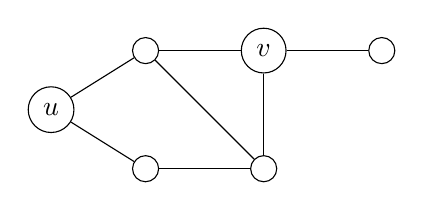
\begin{tikzpicture}
        \node[circle,draw] (v0) at (-0.2,0.75) {$u$};
        \node[circle,draw] (v1) at (1,1.5) {};
        \node[circle,draw] (v2) at (1,0) {};
        \node[circle,draw] (v3) at (2.5,1.5) {$v$};
        \node[circle,draw] (v4) at (2.5,0) {};
        \node[circle,draw] (v5) at (4,1.5) {};

        \draw (v0) -- (v1);
        \draw (v0) -- (v2);
        \draw (v1) -- (v3);
        \draw (v1) -- (v4);
        \draw (v2) -- (v4);
        \draw (v3) -- (v4);
        \draw (v3) -- (v5);
    \end{tikzpicture}
\end{center}

I will show step for step how we will encode this input graph as a Colored Graph.
First, to overcome the problem mentioned before of arbitrary degree, we will encode every vertex of the input as ring of nodes.
Then each node in a given vertex ring is only incident to one edge of the original graph.
The ring nodes are connected with black edges while the edges between vertices are green.

\begin{center}
    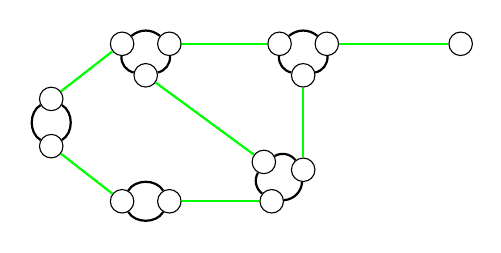
\begin{tikzpicture}
        \node[circle,draw,inner sep=3pt] (v00) at (-0.2,0.7) {};
        \node[circle,draw,inner sep=3pt] (v01) at (-0.2,1.3) {};
        \node[circle,draw,inner sep=3pt] (v10) at (0.7,2) {};
        \node[circle,draw,inner sep=3pt] (v11) at (1,1.6) {};
        \node[circle,draw,inner sep=3pt] (v12) at (1.3,2) {};
        \node[circle,draw,inner sep=3pt] (v20) at (0.7,0) {};
        \node[circle,draw,inner sep=3pt] (v21) at (1.3,0) {};
        \node[circle,draw,inner sep=3pt] (v30) at (2.7,2) {};
        \node[circle,draw,inner sep=3pt] (v31) at (3,1.6) {};
        \node[circle,draw,inner sep=3pt] (v32) at (3.3,2) {};
        \node[circle,draw,inner sep=3pt] (v40) at (2.6,0) {};
        \node[circle,draw,inner sep=3pt] (v41) at (2.5,0.5) {};
        \node[circle,draw,inner sep=3pt] (v42) at (3,0.4) {};
        \node[circle,draw,inner sep=3pt] (v5) at (5,2) {};

        \draw[thick,bend right=60] (v00) to (v01);
        \draw[thick,bend left=60] (v00) to (v01);
        \draw[thick,bend left=40] (v10) to (v12);
        \draw[thick,bend left=40] (v12) to (v11);
        \draw[thick,bend left=40] (v11) to (v10);
        \draw[thick,bend right=60] (v20) to (v21);
        \draw[thick,bend left=60] (v20) to (v21);
        \draw[thick,bend left=40] (v30) to (v32);
        \draw[thick,bend left=40] (v32) to (v31);
        \draw[thick,bend left=40] (v31) to (v30);
        \draw[thick,bend left=40] (v40) to (v41);
        \draw[thick,bend left=40] (v41) to (v42);
        \draw[thick,bend left=40] (v42) to (v40);

        \draw[thick,green] (v00) -- (v20);
        \draw[thick,green] (v01) -- (v10);
        \draw[thick,green] (v12) -- (v30);
        \draw[thick,green] (v11) -- (v41);
        \draw[thick,green] (v21) -- (v40);
        \draw[thick,green] (v31) -- (v42);
        \draw[thick,green] (v32) -- (v5);
    \end{tikzpicture}
\end{center}

Because we will perform a form of BFS on the graph we need some sense of direntionality in the edges.
Not in the sense that we can only go along the in one direction, but in the sense that we remember from which side an update originated.
To to this we will insert a node inbetween each edge.
This also result in no more multi-edges.
We will also extend any node of degree one (so for our example graph the node on the right) with an additional node so that it too becomes a proper ring.
That way the rules will get slightly simpler.

\begin{center}
    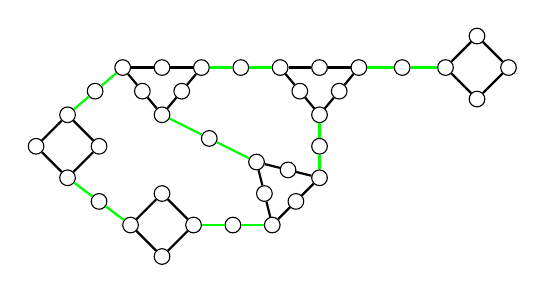
\begin{tikzpicture}
        \node[circle,draw,inner sep=2pt] (v00) at (-0.2,0.6) {};
        \node[circle,draw,inner sep=2pt] (v01) at (-0.2,1.4) {};
        \node[circle,draw,inner sep=2pt] (v02) at (-0.6,1) {};
        \node[circle,draw,inner sep=2pt] (v03) at (0.2,1) {};

        \node[circle,draw,inner sep=2pt] (c01) at (0.15,1.7) {};

        \node[circle,draw,inner sep=2pt] (v10) at (0.5,2) {};
        \node[circle,draw,inner sep=2pt] (v11) at (1,1.4) {};
        \node[circle,draw,inner sep=2pt] (v12) at (1.5,2) {};
        \node[circle,draw,inner sep=2pt] (v13) at (0.75,1.7) {};
        \node[circle,draw,inner sep=2pt] (v14) at (1.25,1.7) {};
        \node[circle,draw,inner sep=2pt] (v15) at (1,2) {};

        \node[circle,draw,inner sep=2pt] (c02) at (0.2,0.3) {};

        \node[circle,draw,inner sep=2pt] (v20) at (0.6,0) {};
        \node[circle,draw,inner sep=2pt] (v21) at (1.4,0) {};
        \node[circle,draw,inner sep=2pt] (v22) at (1,-0.4) {};
        \node[circle,draw,inner sep=2pt] (v23) at (1,0.4) {};

        \node[circle,draw,inner sep=2pt] (c13) at (2,2) {};

        \node[circle,draw,inner sep=2pt] (v30) at (2.5,2) {};
        \node[circle,draw,inner sep=2pt] (v31) at (3,1.4) {};
        \node[circle,draw,inner sep=2pt] (v32) at (3.5,2) {};
        \node[circle,draw,inner sep=2pt] (v33) at (2.75,1.7) {};
        \node[circle,draw,inner sep=2pt] (v34) at (3.25,1.7) {};
        \node[circle,draw,inner sep=2pt] (v35) at (3,2) {};

        \node[circle,draw,inner sep=2pt] (c14) at (1.6,1.1) {};
        \node[circle,draw,inner sep=2pt] (c24) at (1.9,0) {};
        \node[circle,draw,inner sep=2pt] (c34) at (3,1) {};
    
        \node[circle,draw,inner sep=2pt] (v40) at (2.4,0) {};
        \node[circle,draw,inner sep=2pt] (v41) at (2.2,0.8) {};
        \node[circle,draw,inner sep=2pt] (v42) at (3,0.6) {};
        \node[circle,draw,inner sep=2pt] (v43) at (2.3,0.4) {};
        \node[circle,draw,inner sep=2pt] (v44) at (2.6,0.7) {};
        \node[circle,draw,inner sep=2pt] (v45) at (2.7,0.3) {};

        \node[circle,draw,inner sep=2pt] (c35) at (4.05,2) {};

        \node[circle,draw,inner sep=2pt] (v50) at (5,1.6) {};
        \node[circle,draw,inner sep=2pt] (v51) at (5,2.4) {};
        \node[circle,draw,inner sep=2pt] (v52) at (4.6,2) {};
        \node[circle,draw,inner sep=2pt] (v53) at (5.4,2) {};

        \draw[thick] (v00) to (v02);
        \draw[thick] (v02) to (v01);
        \draw[thick] (v01) to (v03);
        \draw[thick] (v03) to (v00);

        \draw[thick] (v10) to (v13);
        \draw[thick] (v13) to (v11);
        \draw[thick] (v11) to (v14);
        \draw[thick] (v14) to (v12);
        \draw[thick] (v12) to (v15);
        \draw[thick] (v15) to (v10);

        \draw[thick] (v20) to (v22);
        \draw[thick] (v22) to (v21);
        \draw[thick] (v21) to (v23);
        \draw[thick] (v23) to (v20);

        \draw[thick] (v30) to (v33);
        \draw[thick] (v33) to (v31);
        \draw[thick] (v31) to (v34);
        \draw[thick] (v34) to (v32);
        \draw[thick] (v32) to (v35);
        \draw[thick] (v35) to (v30);

        \draw[thick] (v40) to (v43);
        \draw[thick] (v43) to (v41);
        \draw[thick] (v41) to (v44);
        \draw[thick] (v44) to (v42);
        \draw[thick] (v42) to (v45);
        \draw[thick] (v45) to (v40);

        \draw[thick] (v50) to (v52);
        \draw[thick] (v52) to (v51);
        \draw[thick] (v51) to (v53);
        \draw[thick] (v53) to (v50);

        \draw[thick,green] (v00) -- (c02);
        \draw[thick,green] (c02) -- (v20);

        \draw[thick,green] (v01) -- (c01);
        \draw[thick,green] (c01) -- (v10);

        \draw[thick,green] (v12) -- (c13);
        \draw[thick,green] (c13) -- (v30);

        \draw[thick,green] (v11) -- (c14);
        \draw[thick,green] (c14) -- (v41);

        \draw[thick,green] (v21) -- (c24);
        \draw[thick,green] (c24) -- (v40);

        \draw[thick,green] (v31) -- (c34);
        \draw[thick,green] (c34) -- (v42);

        \draw[thick,green] (v32) -- (c35);
        \draw[thick,green] (c35) -- (v52);
    \end{tikzpicture}
\end{center}

As a last step we will mark the start end end vertex.
To do this we insert a node into each ring and connect the start vertex to a dummy vertex with red and the goal vertex with blue.

\begin{center}
    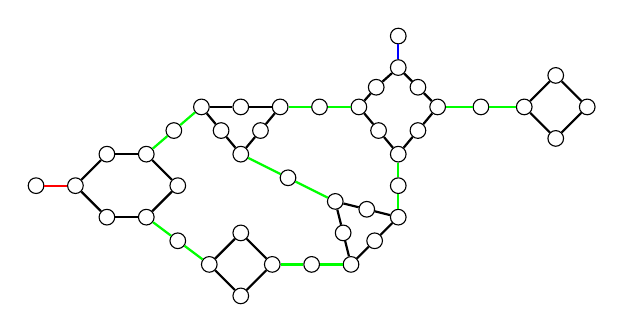
\begin{tikzpicture}
        \node[circle,draw,inner sep=2pt] (v00) at (-0.2,0.6) {};
        \node[circle,draw,inner sep=2pt] (v01) at (-0.2,1.4) {};
        \node[circle,draw,inner sep=2pt] (v02) at (-0.7,1.4) {};
        \node[circle,draw,inner sep=2pt] (v03) at (0.2,1) {};
        \node[circle,draw,inner sep=2pt] (v04) at (-0.7,0.6) {};
        \node[circle,draw,inner sep=2pt] (v05) at (-1.1,1) {};

        \node[circle,draw,inner sep=2pt] (s) at (-1.6,1) {};

        \node[circle,draw,inner sep=2pt] (c01) at (0.15,1.7) {};

        \node[circle,draw,inner sep=2pt] (v10) at (0.5,2) {};
        \node[circle,draw,inner sep=2pt] (v11) at (1,1.4) {};
        \node[circle,draw,inner sep=2pt] (v12) at (1.5,2) {};
        \node[circle,draw,inner sep=2pt] (v13) at (0.75,1.7) {};
        \node[circle,draw,inner sep=2pt] (v14) at (1.25,1.7) {};
        \node[circle,draw,inner sep=2pt] (v15) at (1,2) {};

        \node[circle,draw,inner sep=2pt] (c02) at (0.2,0.3) {};

        \node[circle,draw,inner sep=2pt] (v20) at (0.6,0) {};
        \node[circle,draw,inner sep=2pt] (v21) at (1.4,0) {};
        \node[circle,draw,inner sep=2pt] (v22) at (1,-0.4) {};
        \node[circle,draw,inner sep=2pt] (v23) at (1,0.4) {};

        \node[circle,draw,inner sep=2pt] (c13) at (2,2) {};

        \node[circle,draw,inner sep=2pt] (v30) at (2.5,2) {};
        \node[circle,draw,inner sep=2pt] (v31) at (3,1.4) {};
        \node[circle,draw,inner sep=2pt] (v32) at (3.5,2) {};
        \node[circle,draw,inner sep=2pt] (v33) at (2.75,1.7) {};
        \node[circle,draw,inner sep=2pt] (v34) at (3.25,1.7) {};
        \node[circle,draw,inner sep=2pt] (v35) at (3.25,2.25) {};
        \node[circle,draw,inner sep=2pt] (v36) at (3,2.5) {};
        \node[circle,draw,inner sep=2pt] (v37) at (2.72,2.25) {};

        \node[circle,draw,inner sep=2pt] (g) at (3,2.9) {};

        \node[circle,draw,inner sep=2pt] (c14) at (1.6,1.1) {};
        \node[circle,draw,inner sep=2pt] (c24) at (1.9,0) {};
        \node[circle,draw,inner sep=2pt] (c34) at (3,1) {};
    
        \node[circle,draw,inner sep=2pt] (v40) at (2.4,0) {};
        \node[circle,draw,inner sep=2pt] (v41) at (2.2,0.8) {};
        \node[circle,draw,inner sep=2pt] (v42) at (3,0.6) {};
        \node[circle,draw,inner sep=2pt] (v43) at (2.3,0.4) {};
        \node[circle,draw,inner sep=2pt] (v44) at (2.6,0.7) {};
        \node[circle,draw,inner sep=2pt] (v45) at (2.7,0.3) {};
        
        \node[circle,draw,inner sep=2pt] (c35) at (4.05,2) {};

        \node[circle,draw,inner sep=2pt] (v50) at (5,1.6) {};
        \node[circle,draw,inner sep=2pt] (v51) at (5,2.4) {};
        \node[circle,draw,inner sep=2pt] (v52) at (4.6,2) {};
        \node[circle,draw,inner sep=2pt] (v53) at (5.4,2) {};

        \draw[thick,red] (s) to (v05);

        \draw[thick] (v00) to (v04);
        \draw[thick] (v05) to (v04);
        \draw[thick] (v02) to (v05);
        \draw[thick] (v02) to (v01);
        \draw[thick] (v01) to (v03);
        \draw[thick] (v03) to (v00);

        \draw[thick] (v10) to (v13);
        \draw[thick] (v13) to (v11);
        \draw[thick] (v11) to (v14);
        \draw[thick] (v14) to (v12);
        \draw[thick] (v12) to (v15);
        \draw[thick] (v15) to (v10);

        \draw[thick] (v20) to (v22);
        \draw[thick] (v22) to (v21);
        \draw[thick] (v21) to (v23);
        \draw[thick] (v23) to (v20);

        \draw[thick] (v30) to (v33);
        \draw[thick] (v33) to (v31);
        \draw[thick] (v31) to (v34);
        \draw[thick] (v34) to (v32);
        \draw[thick] (v32) to (v35);
        \draw[thick] (v35) to (v36);
        \draw[thick] (v36) to (v37);
        \draw[thick] (v37) to (v30);

        \draw[thick, blue] (v36) to (g);

        \draw[thick] (v40) to (v43);
        \draw[thick] (v43) to (v41);
        \draw[thick] (v41) to (v44);
        \draw[thick] (v44) to (v42);
        \draw[thick] (v42) to (v45);
        \draw[thick] (v45) to (v40);

        \draw[thick] (v50) to (v52);
        \draw[thick] (v52) to (v51);
        \draw[thick] (v51) to (v53);
        \draw[thick] (v53) to (v50);

        \draw[thick,green] (v00) -- (c02);
        \draw[thick,green] (c02) -- (v20);

        \draw[thick,green] (v01) -- (c01);
        \draw[thick,green] (c01) -- (v10);

        \draw[thick,green] (v12) -- (c13);
        \draw[thick,green] (c13) -- (v30);

        \draw[thick,green] (v11) -- (c14);
        \draw[thick,green] (c14) -- (v41);

        \draw[thick,green] (v21) -- (c24);
        \draw[thick,green] (c24) -- (v40);

        \draw[thick,green] (v31) -- (c34);
        \draw[thick,green] (c34) -- (v42);

        \draw[thick,green] (v32) -- (c35);
        \draw[thick,green] (c35) -- (v52);
    \end{tikzpicture}
\end{center}

Our algorithm to find the shortest distance will go as follows.
We will have a counter at the start node and in each iteration we will increase the counter by one and then explore the graph extending our expored areas by taking one more green edge.
Then in the iteration where we find the goal node marked with blue we know that our counter is the distance to it.

Now I will describe the rules that are needed for the algorithm.
I will interleave the rules with showing what they do on our example.
First, we start of with the following rule:

\begin{center}
    \begin{tikzpicture}
        \begin{scope}[xshift=-2cm]
            \node[circle,draw,fill] (A) at (0, 0) {};
            \node[circle,draw] (B) at (-1,0) {};
            \node[circle,draw] (C) at (0.7,0.7) {};
            \node[circle,draw] (D) at (0.7,-0.7) {};
            
            \draw[thick,red] (A) -- (B);
            \draw[thick] (A) -- (C);
            \draw[thick] (A) -- (D);
        \end{scope}
    
        \draw [line width=1pt, double distance=3pt, arrows = {-Latex[length=0pt 3 0]}] (-0.5,0) -- node[above] {(1)} (0.5,0);
        
        \begin{scope}[xshift=3.2cm]
            \node[circle,draw,fill] (A) at (0, 0) {};
            \node[circle,draw] (B) at (-1,0) {};
            \node[circle,draw] (C) at (0.7,0.7) {};
            \node[circle,draw] (D) at (0.7,-0.7) {};
            \node[circle,draw,fill] (E) at (-2,0) {};
            
            \draw[thick,pink] (A) -- (B);
            \draw[thick,yellow] (A) -- (C);
            \draw[thick,yellow] (A) -- (D);
            \draw[thick,blue] (B) -- (E);
        \end{scope}
    \end{tikzpicture}
\end{center}

This rule will start our algorithm by initializing the counter to one (the blue edge), and marking the two neighboring edges ready for exploration (yellow).

\begin{center}
    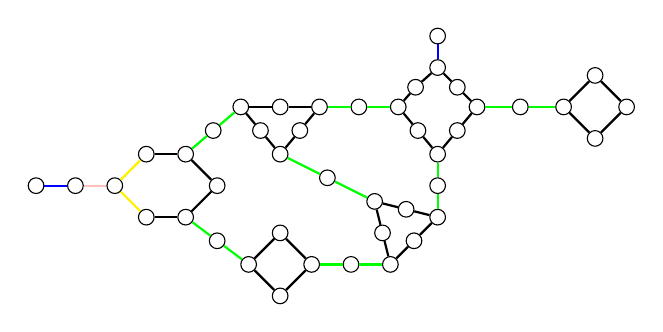
\begin{tikzpicture}
        \node[circle,draw,inner sep=2pt] (v00) at (-0.2,0.6) {};
        \node[circle,draw,inner sep=2pt] (v01) at (-0.2,1.4) {};
        \node[circle,draw,inner sep=2pt] (v02) at (-0.7,1.4) {};
        \node[circle,draw,inner sep=2pt] (v03) at (0.2,1) {};
        \node[circle,draw,inner sep=2pt] (v04) at (-0.7,0.6) {};
        \node[circle,draw,inner sep=2pt] (v05) at (-1.1,1) {};

        \node[circle,draw,inner sep=2pt] (n1) at (-2.1,1) {};
        \node[circle,draw,inner sep=2pt] (s) at (-1.6,1) {};

        \node[circle,draw,inner sep=2pt] (c01) at (0.15,1.7) {};

        \node[circle,draw,inner sep=2pt] (v10) at (0.5,2) {};
        \node[circle,draw,inner sep=2pt] (v11) at (1,1.4) {};
        \node[circle,draw,inner sep=2pt] (v12) at (1.5,2) {};
        \node[circle,draw,inner sep=2pt] (v13) at (0.75,1.7) {};
        \node[circle,draw,inner sep=2pt] (v14) at (1.25,1.7) {};
        \node[circle,draw,inner sep=2pt] (v15) at (1,2) {};

        \node[circle,draw,inner sep=2pt] (c02) at (0.2,0.3) {};

        \node[circle,draw,inner sep=2pt] (v20) at (0.6,0) {};
        \node[circle,draw,inner sep=2pt] (v21) at (1.4,0) {};
        \node[circle,draw,inner sep=2pt] (v22) at (1,-0.4) {};
        \node[circle,draw,inner sep=2pt] (v23) at (1,0.4) {};

        \node[circle,draw,inner sep=2pt] (c13) at (2,2) {};

        \node[circle,draw,inner sep=2pt] (v30) at (2.5,2) {};
        \node[circle,draw,inner sep=2pt] (v31) at (3,1.4) {};
        \node[circle,draw,inner sep=2pt] (v32) at (3.5,2) {};
        \node[circle,draw,inner sep=2pt] (v33) at (2.75,1.7) {};
        \node[circle,draw,inner sep=2pt] (v34) at (3.25,1.7) {};
        \node[circle,draw,inner sep=2pt] (v35) at (3.25,2.25) {};
        \node[circle,draw,inner sep=2pt] (v36) at (3,2.5) {};
        \node[circle,draw,inner sep=2pt] (v37) at (2.72,2.25) {};

        \node[circle,draw,inner sep=2pt] (g) at (3,2.9) {};

        \node[circle,draw,inner sep=2pt] (c14) at (1.6,1.1) {};
        \node[circle,draw,inner sep=2pt] (c24) at (1.9,0) {};
        \node[circle,draw,inner sep=2pt] (c34) at (3,1) {};
    
        \node[circle,draw,inner sep=2pt] (v40) at (2.4,0) {};
        \node[circle,draw,inner sep=2pt] (v41) at (2.2,0.8) {};
        \node[circle,draw,inner sep=2pt] (v42) at (3,0.6) {};
        \node[circle,draw,inner sep=2pt] (v43) at (2.3,0.4) {};
        \node[circle,draw,inner sep=2pt] (v44) at (2.6,0.7) {};
        \node[circle,draw,inner sep=2pt] (v45) at (2.7,0.3) {};
        
        \node[circle,draw,inner sep=2pt] (c35) at (4.05,2) {};

        \node[circle,draw,inner sep=2pt] (v50) at (5,1.6) {};
        \node[circle,draw,inner sep=2pt] (v51) at (5,2.4) {};
        \node[circle,draw,inner sep=2pt] (v52) at (4.6,2) {};
        \node[circle,draw,inner sep=2pt] (v53) at (5.4,2) {};

        \draw[thick,pink] (s) to (v05);
        \draw[thick,blue] (n1) to (s);

        \draw[thick] (v00) to (v04);
        \draw[thick,yellow] (v05) to (v04);
        \draw[thick,yellow] (v02) to (v05);
        \draw[thick] (v02) to (v01);
        \draw[thick] (v01) to (v03);
        \draw[thick] (v03) to (v00);

        \draw[thick] (v10) to (v13);
        \draw[thick] (v13) to (v11);
        \draw[thick] (v11) to (v14);
        \draw[thick] (v14) to (v12);
        \draw[thick] (v12) to (v15);
        \draw[thick] (v15) to (v10);

        \draw[thick] (v20) to (v22);
        \draw[thick] (v22) to (v21);
        \draw[thick] (v21) to (v23);
        \draw[thick] (v23) to (v20);

        \draw[thick] (v30) to (v33);
        \draw[thick] (v33) to (v31);
        \draw[thick] (v31) to (v34);
        \draw[thick] (v34) to (v32);
        \draw[thick] (v32) to (v35);
        \draw[thick] (v35) to (v36);
        \draw[thick] (v36) to (v37);
        \draw[thick] (v37) to (v30);

        \draw[thick, blue] (v36) to (g);

        \draw[thick] (v40) to (v43);
        \draw[thick] (v43) to (v41);
        \draw[thick] (v41) to (v44);
        \draw[thick] (v44) to (v42);
        \draw[thick] (v42) to (v45);
        \draw[thick] (v45) to (v40);

        \draw[thick] (v50) to (v52);
        \draw[thick] (v52) to (v51);
        \draw[thick] (v51) to (v53);
        \draw[thick] (v53) to (v50);

        \draw[thick,green] (v00) -- (c02);
        \draw[thick,green] (c02) -- (v20);

        \draw[thick,green] (v01) -- (c01);
        \draw[thick,green] (c01) -- (v10);

        \draw[thick,green] (v12) -- (c13);
        \draw[thick,green] (c13) -- (v30);

        \draw[thick,green] (v11) -- (c14);
        \draw[thick,green] (c14) -- (v41);

        \draw[thick,green] (v21) -- (c24);
        \draw[thick,green] (c24) -- (v40);

        \draw[thick,green] (v31) -- (c34);
        \draw[thick,green] (c34) -- (v42);

        \draw[thick,green] (v32) -- (c35);
        \draw[thick,green] (c35) -- (v52);
    \end{tikzpicture}
\end{center}

Then we use the following rules to go through all black edges and whenever we reach a green edge we change it to dark green.
This is done so that in the next iteration, we know we already visited that edge once and can now explore the neighboring vertex.

\begin{center}
    \begin{tikzpicture}
        % SplitRule(
        %     name="Propagate update",
        %     input={"yellow": 1, "black": 1},
        %     node1_connection={"yellow": "yellow", "black": "orange"},
        %     node2_connection={},
        % ),
        \begin{scope}[xshift=-4cm]
            \begin{scope}[xshift=-2cm]
                \node[circle,draw,fill] (A) at (0, 0) {};
                \node[circle,draw] (B) at (-1,0) {};
                \node[circle,draw] (D) at (1,0) {};
                
                \draw[thick,yellow] (A) -- (B);
                \draw[thick,black] (A) -- (D);
            \end{scope}
        
            \draw [line width=1pt, double distance=3pt, arrows = {-Latex[length=0pt 3 0]}] (-0.5,0) -- node[above] {(2)} (0.5,0);
            
            \begin{scope}[xshift=2.2cm]
                \node[circle,draw,fill] (A) at (0, 0) {};
                \node[circle,draw,fill] (A') at (0, 0.5) {};
                \node[circle,draw] (B) at (-1,0) {};
                \node[circle,draw] (D) at (1,0) {};
                
                \draw[thick,yellow] (A) -- (B);
                \draw[thick,orange] (A) -- (D);
            \end{scope}
        \end{scope}

        % SplitRule(
        %     name="Colliding updated",
        %     input={"yellow": 2},
        %     node1_connection={"yellow": "black"},
        %     node2_connection={},
        % ),
        \begin{scope}[xshift=4cm]
            \begin{scope}[xshift=-2cm]
                \node[circle,draw,fill] (A) at (0, 0) {};
                \node[circle,draw] (B) at (-1,0) {};
                \node[circle,draw] (D) at (1,0) {};
                
                \draw[thick,yellow] (A) -- (B);
                \draw[thick,yellow] (A) -- (D);
            \end{scope}
        
            \draw [line width=1pt, double distance=3pt, arrows = {-Latex[length=0pt 3 0]}] (-0.5,0) -- node[above] {(3)} (0.5,0);
            
            \begin{scope}[xshift=2.2cm]
                \node[circle,draw,fill] (A) at (0, 0) {};
                \node[circle,draw,fill] (A') at (0, 0.5) {};
                \node[circle,draw] (B) at (-1,0) {};
                \node[circle,draw] (D) at (1,0) {};
                
                \draw[thick,black] (A) -- (B);
                \draw[thick,black] (A) -- (D);
            \end{scope}
        \end{scope}
    \end{tikzpicture}

    \vspace*{0.5cm}

    \begin{tikzpicture}
        % SplitRule(
        %     name="Update next nodes",
        %     input={"orange": 1, "black": 2},
        %     node1_connection={"orange": "purple", "black": "yellow"},
        %     node2_connection={},
        % ),
        \begin{scope}[xshift=-4cm]
            \begin{scope}[xshift=-2cm]
                \node[circle,draw,fill] (A) at (0, 0) {};
                \node[circle,draw] (B) at (-1,0) {};
                \node[circle,draw] (C) at (0.7,0.7) {};
                \node[circle,draw] (D) at (0.7,-0.7) {};
                
                \draw[thick,orange] (A) -- (B);
                \draw[thick,black] (A) -- (C);
                \draw[thick,black] (A) -- (D);
            \end{scope}
        
            \draw [line width=1pt, double distance=3pt, arrows = {-Latex[length=0pt 3 0]}] (-0.5,0) -- node[above] {(4)} (0.5,0);
            
            \begin{scope}[xshift=2.2cm]
                \node[circle,draw,fill] (A') at (-0.3, 0.5) {};
                \node[circle,draw,fill] (A) at (0, 0) {};
                \node[circle,draw] (B) at (-1,0) {};
                \node[circle,draw] (C) at (0.7,0.7) {};
                \node[circle,draw] (D) at (0.7,-0.7) {};
                
                \draw[thick,purple] (A) -- (B);
                \draw[thick,yellow] (A) -- (C);
                \draw[thick,yellow] (A) -- (D);
            \end{scope}
        \end{scope}

        % SplitRule(
        %     name="Expand reach",
        %     input={"orange": 1, "green": 1, "black": 1},
        %     node1_connection={"orange": "purple", "green": "lime", "black": "yellow"},
        %     node2_connection={},
        % ),
        \begin{scope}[xshift=4cm]
            \begin{scope}[xshift=-2cm]
                \node[circle,draw,fill] (A) at (0, 0) {};
                \node[circle,draw] (B) at (-1,0) {};
                \node[circle,draw] (C) at (0.7,0.7) {};
                \node[circle,draw] (D) at (0.7,-0.7) {};
                
                \draw[thick,orange] (A) -- (B);
                \draw[thick,green] (A) -- (C);
                \draw[thick,black] (A) -- (D);
            \end{scope}
        
            \draw [line width=1pt, double distance=3pt, arrows = {-Latex[length=0pt 3 0]}] (-0.5,0) -- node[above] {(5)} (0.5,0);
            
            \begin{scope}[xshift=2.2cm]
                \node[circle,draw,fill] (A') at (-0.3, 0.5) {};
                \node[circle,draw,fill] (A) at (0, 0) {};
                \node[circle,draw] (B) at (-1,0) {};
                \node[circle,draw] (C) at (0.7,0.7) {};
                \node[circle,draw] (D) at (0.7,-0.7) {};
                
                \draw[thick,purple] (A) -- (B);
                \draw[thick,forestgreen] (A) -- (C);
                \draw[thick,yellow] (A) -- (D);
            \end{scope}
        \end{scope}
    \end{tikzpicture}

    \vspace*{0.5cm}

    \begin{tikzpicture}
        % SplitRule(
        %     name="Expand reach",
        %     input={"orange": 2, "green": 1},
        %     node1_connection={"orange": "olive", "green": "lime"},
        %     node2_connection={},
        % ),
        \begin{scope}[xshift=-4cm]
            \begin{scope}[xshift=-2cm]
                \node[circle,draw,fill] (A) at (0, 0) {};
                \node[circle,draw] (B) at (-1,0) {};
                \node[circle,draw] (C) at (0.7,0.7) {};
                \node[circle,draw] (D) at (0.7,-0.7) {};
                
                \draw[thick,orange] (A) -- (B);
                \draw[thick,orange] (A) -- (C);
                \draw[thick,green] (A) -- (D);
            \end{scope}
        
            \draw [line width=1pt, double distance=3pt, arrows = {-Latex[length=0pt 3 0]}] (-0.5,0) -- node[above] {(6)} (0.5,0);
            
            \begin{scope}[xshift=2.2cm]
                \node[circle,draw,fill] (A') at (-0.3, 0.5) {};
                \node[circle,draw,fill] (A) at (0, 0) {};
                \node[circle,draw] (B) at (-1,0) {};
                \node[circle,draw] (C) at (0.7,0.7) {};
                \node[circle,draw] (D) at (0.7,-0.7) {};
                
                \draw[thick,olive] (A) -- (B);
                \draw[thick,olive] (A) -- (C);
                \draw[thick,forestgreen] (A) -- (D);
            \end{scope}
        \end{scope}

        % DeleteRule
        \begin{scope}[xshift=4cm]
            \begin{scope}[xshift=-1.3cm]
                \node[circle,draw,fill] (A) at (0, 0) {};
            \end{scope}
        
            \draw [line width=1pt, double distance=3pt, arrows = {-Latex[length=0pt 3 0]}] (-0.5,0) -- node[above] {(7)} (0.5,0);
            
            \begin{scope}[xshift=2.2cm]
            \end{scope}
        \end{scope}
    \end{tikzpicture}
\end{center}

Applying these rules allows us to explore the first ring (vertex u).
We alternate yellow and orange so we know from which edge we reached a node (the one marked with orange).
After an orange edge has been created we update the neighboring edges with yellow to expore them (rule (2) and (4)).
If we reach a green edge we don't traverse it yet but mark it with dark green so we know that in the next iteration we can traverse it (rule (5)).
In those 3 rules we will only change the orange edge to a purple one to remember that this vertex has already been updated.
It might happen that a vertex get updated by two sides at the same time.
It these are the only two edges of the node (rule (3)) then we change the edges back to black basically marking them as done.
If there is also a a green edge (rule (6)), we again change the green edge to dark green, but now instead of turning the orange edges purple we turn them to olive.a
This is just an optimisation as olive will mark that the node and all its children are done updating.
Rule (7) just deletes any isolated vertex we generate with the other Split Rules.

When we apply these rules to our example it depends slightly on which order we apply them but it will turn out that it won't matter in the end.
A resulting graph could be like the following.

\begin{center}
    \begin{tikzpicture}
        \node[circle,draw,inner sep=2pt] (v00) at (-0.2,0.6) {};
        \node[circle,draw,inner sep=2pt] (v01) at (-0.2,1.4) {};
        \node[circle,draw,inner sep=2pt] (v02) at (-0.7,1.4) {};
        \node[circle,draw,inner sep=2pt] (v03) at (0.2,1) {};
        \node[circle,draw,inner sep=2pt] (v04) at (-0.7,0.6) {};
        \node[circle,draw,inner sep=2pt] (v05) at (-1.1,1) {};

        \node[circle,draw,inner sep=2pt] (n1) at (-2.1,1) {};
        \node[circle,draw,inner sep=2pt] (s) at (-1.6,1) {};

        \node[circle,draw,inner sep=2pt] (c01) at (0.15,1.7) {};

        \node[circle,draw,inner sep=2pt] (v10) at (0.5,2) {};
        \node[circle,draw,inner sep=2pt] (v11) at (1,1.4) {};
        \node[circle,draw,inner sep=2pt] (v12) at (1.5,2) {};
        \node[circle,draw,inner sep=2pt] (v13) at (0.75,1.7) {};
        \node[circle,draw,inner sep=2pt] (v14) at (1.25,1.7) {};
        \node[circle,draw,inner sep=2pt] (v15) at (1,2) {};

        \node[circle,draw,inner sep=2pt] (c02) at (0.2,0.3) {};

        \node[circle,draw,inner sep=2pt] (v20) at (0.6,0) {};
        \node[circle,draw,inner sep=2pt] (v21) at (1.4,0) {};
        \node[circle,draw,inner sep=2pt] (v22) at (1,-0.4) {};
        \node[circle,draw,inner sep=2pt] (v23) at (1,0.4) {};

        \node[circle,draw,inner sep=2pt] (c13) at (2,2) {};

        \node[circle,draw,inner sep=2pt] (v30) at (2.5,2) {};
        \node[circle,draw,inner sep=2pt] (v31) at (3,1.4) {};
        \node[circle,draw,inner sep=2pt] (v32) at (3.5,2) {};
        \node[circle,draw,inner sep=2pt] (v33) at (2.75,1.7) {};
        \node[circle,draw,inner sep=2pt] (v34) at (3.25,1.7) {};
        \node[circle,draw,inner sep=2pt] (v35) at (3.25,2.25) {};
        \node[circle,draw,inner sep=2pt] (v36) at (3,2.5) {};
        \node[circle,draw,inner sep=2pt] (v37) at (2.72,2.25) {};

        \node[circle,draw,inner sep=2pt] (g) at (3,2.9) {};

        \node[circle,draw,inner sep=2pt] (c14) at (1.6,1.1) {};
        \node[circle,draw,inner sep=2pt] (c24) at (1.9,0) {};
        \node[circle,draw,inner sep=2pt] (c34) at (3,1) {};
    
        \node[circle,draw,inner sep=2pt] (v40) at (2.4,0) {};
        \node[circle,draw,inner sep=2pt] (v41) at (2.2,0.8) {};
        \node[circle,draw,inner sep=2pt] (v42) at (3,0.6) {};
        \node[circle,draw,inner sep=2pt] (v43) at (2.3,0.4) {};
        \node[circle,draw,inner sep=2pt] (v44) at (2.6,0.7) {};
        \node[circle,draw,inner sep=2pt] (v45) at (2.7,0.3) {};
        
        \node[circle,draw,inner sep=2pt] (c35) at (4.05,2) {};

        \node[circle,draw,inner sep=2pt] (v50) at (5,1.6) {};
        \node[circle,draw,inner sep=2pt] (v51) at (5,2.4) {};
        \node[circle,draw,inner sep=2pt] (v52) at (4.6,2) {};
        \node[circle,draw,inner sep=2pt] (v53) at (5.4,2) {};

        \draw[thick,pink] (s) to (v05);
        \draw[thick,blue] (n1) to (s);

        \draw[thick,olive] (v00) to (v04);
        \draw[thick,yellow] (v05) to (v04);
        \draw[thick,yellow] (v02) to (v05);
        \draw[thick,purple] (v02) to (v01);
        \draw[thick,yellow] (v01) to (v03);
        \draw[thick,olive] (v03) to (v00);

        \draw[thick] (v10) to (v13);
        \draw[thick] (v13) to (v11);
        \draw[thick] (v11) to (v14);
        \draw[thick] (v14) to (v12);
        \draw[thick] (v12) to (v15);
        \draw[thick] (v15) to (v10);

        \draw[thick] (v20) to (v22);
        \draw[thick] (v22) to (v21);
        \draw[thick] (v21) to (v23);
        \draw[thick] (v23) to (v20);

        \draw[thick] (v30) to (v33);
        \draw[thick] (v33) to (v31);
        \draw[thick] (v31) to (v34);
        \draw[thick] (v34) to (v32);
        \draw[thick] (v32) to (v35);
        \draw[thick] (v35) to (v36);
        \draw[thick] (v36) to (v37);
        \draw[thick] (v37) to (v30);

        \draw[thick, blue] (v36) to (g);

        \draw[thick] (v40) to (v43);
        \draw[thick] (v43) to (v41);
        \draw[thick] (v41) to (v44);
        \draw[thick] (v44) to (v42);
        \draw[thick] (v42) to (v45);
        \draw[thick] (v45) to (v40);

        \draw[thick] (v50) to (v52);
        \draw[thick] (v52) to (v51);
        \draw[thick] (v51) to (v53);
        \draw[thick] (v53) to (v50);

        \draw[thick,forestgreen] (v00) -- (c02);
        \draw[thick,green] (c02) -- (v20);

        \draw[thick,forestgreen] (v01) -- (c01);
        \draw[thick,green] (c01) -- (v10);

        \draw[thick,green] (v12) -- (c13);
        \draw[thick,green] (c13) -- (v30);

        \draw[thick,green] (v11) -- (c14);
        \draw[thick,green] (c14) -- (v41);

        \draw[thick,green] (v21) -- (c24);
        \draw[thick,green] (c24) -- (v40);

        \draw[thick,green] (v31) -- (c34);
        \draw[thick,green] (c34) -- (v42);

        \draw[thick,green] (v32) -- (c35);
        \draw[thick,green] (c35) -- (v52);
    \end{tikzpicture}
\end{center}

This iteration explored all vertices that have distance 0 from $u$, namely, just the ring of $u$.
We will now want to backtrace all our expored edges to set up the graph for the next iteration.
For this we will need the following rules.

\begin{center}
    \begin{tikzpicture}
        % SplitRule(
        %     name="Backtrace edge",
        %     input={"yellow": 1, "olive": 1},
        %     node1_connection={"yellow": "black", "olive": "black"},
        %     node2_connection={},
        % ),
        \begin{scope}[xshift=-4cm]
            \begin{scope}[xshift=-2cm]
                \node[circle,draw,fill] (A) at (0, 0) {};
                \node[circle,draw] (B) at (-1,0) {};
                \node[circle,draw] (D) at (1,0) {};
                
                \draw[thick,yellow] (A) -- (B);
                \draw[thick,olive] (A) -- (D);
            \end{scope}
        
            \draw [line width=1pt, double distance=3pt, arrows = {-Latex[length=0pt 3 0]}] (-0.5,0) -- node[above] {(8)} (0.5,0);
            
            \begin{scope}[xshift=2.2cm]
                \node[circle,draw,fill] (A) at (0, 0) {};
                \node[circle,draw,fill] (A') at (0, 0.5) {};
                \node[circle,draw] (B) at (-1,0) {};
                \node[circle,draw] (D) at (1,0) {};
                
                \draw[thick,black] (A) -- (B);
                \draw[thick,black] (A) -- (D);
            \end{scope}
        \end{scope}

        % SplitRule(
        %     name="Done updating (4)",
        %     input={"black": 1, "purple": 1, "lime": 1},
        %     node1_connection={"black": "black", "purple": "olive", "lime": "lime"},
        %     node2_connection={},
        % ),
        \begin{scope}[xshift=4cm]
            \begin{scope}[xshift=-2cm]
                \node[circle,draw,fill] (A) at (0, 0) {};
                \node[circle,draw] (B) at (-1,0) {};
                \node[circle,draw] (C) at (0.7,0.7) {};
                \node[circle,draw] (D) at (0.7,-0.7) {};
                
                \draw[thick,purple] (A) -- (B);
                \draw[thick,forestgreen] (A) -- (C);
                \draw[thick,black] (A) -- (D);
            \end{scope}
        
            \draw [line width=1pt, double distance=3pt, arrows = {-Latex[length=0pt 3 0]}] (-0.5,0) -- node[above] {(9)} (0.5,0);
            
            \begin{scope}[xshift=2.2cm]
                \node[circle,draw,fill] (A') at (-0.3, 0.5) {};
                \node[circle,draw,fill] (A) at (0, 0) {};
                \node[circle,draw] (B) at (-1,0) {};
                \node[circle,draw] (C) at (0.7,0.7) {};
                \node[circle,draw] (D) at (0.7,-0.7) {};
                
                \draw[thick,olive] (A) -- (B);
                \draw[thick,forestgreen] (A) -- (C);
                \draw[thick,black] (A) -- (D);
            \end{scope}
        \end{scope}
    \end{tikzpicture}
\end{center}

These two rules will backtrace the explored vertices and after applying them to our example graph we will get the following graph.

\begin{center}
    \begin{tikzpicture}
        \node[circle,draw,inner sep=2pt] (v00) at (-0.2,0.6) {};
        \node[circle,draw,inner sep=2pt] (v01) at (-0.2,1.4) {};
        \node[circle,draw,inner sep=2pt] (v02) at (-0.7,1.4) {};
        \node[circle,draw,inner sep=2pt] (v03) at (0.2,1) {};
        \node[circle,draw,inner sep=2pt] (v04) at (-0.7,0.6) {};
        \node[circle,draw,inner sep=2pt] (v05) at (-1.1,1) {};

        \node[circle,draw,inner sep=2pt] (n1) at (-2.1,1) {};
        \node[circle,draw,inner sep=2pt] (s) at (-1.6,1) {};

        \node[circle,draw,inner sep=2pt] (c01) at (0.15,1.7) {};

        \node[circle,draw,inner sep=2pt] (v10) at (0.5,2) {};
        \node[circle,draw,inner sep=2pt] (v11) at (1,1.4) {};
        \node[circle,draw,inner sep=2pt] (v12) at (1.5,2) {};
        \node[circle,draw,inner sep=2pt] (v13) at (0.75,1.7) {};
        \node[circle,draw,inner sep=2pt] (v14) at (1.25,1.7) {};
        \node[circle,draw,inner sep=2pt] (v15) at (1,2) {};

        \node[circle,draw,inner sep=2pt] (c02) at (0.2,0.3) {};

        \node[circle,draw,inner sep=2pt] (v20) at (0.6,0) {};
        \node[circle,draw,inner sep=2pt] (v21) at (1.4,0) {};
        \node[circle,draw,inner sep=2pt] (v22) at (1,-0.4) {};
        \node[circle,draw,inner sep=2pt] (v23) at (1,0.4) {};

        \node[circle,draw,inner sep=2pt] (c13) at (2,2) {};

        \node[circle,draw,inner sep=2pt] (v30) at (2.5,2) {};
        \node[circle,draw,inner sep=2pt] (v31) at (3,1.4) {};
        \node[circle,draw,inner sep=2pt] (v32) at (3.5,2) {};
        \node[circle,draw,inner sep=2pt] (v33) at (2.75,1.7) {};
        \node[circle,draw,inner sep=2pt] (v34) at (3.25,1.7) {};
        \node[circle,draw,inner sep=2pt] (v35) at (3.25,2.25) {};
        \node[circle,draw,inner sep=2pt] (v36) at (3,2.5) {};
        \node[circle,draw,inner sep=2pt] (v37) at (2.72,2.25) {};

        \node[circle,draw,inner sep=2pt] (g) at (3,2.9) {};

        \node[circle,draw,inner sep=2pt] (c14) at (1.6,1.1) {};
        \node[circle,draw,inner sep=2pt] (c24) at (1.9,0) {};
        \node[circle,draw,inner sep=2pt] (c34) at (3,1) {};
    
        \node[circle,draw,inner sep=2pt] (v40) at (2.4,0) {};
        \node[circle,draw,inner sep=2pt] (v41) at (2.2,0.8) {};
        \node[circle,draw,inner sep=2pt] (v42) at (3,0.6) {};
        \node[circle,draw,inner sep=2pt] (v43) at (2.3,0.4) {};
        \node[circle,draw,inner sep=2pt] (v44) at (2.6,0.7) {};
        \node[circle,draw,inner sep=2pt] (v45) at (2.7,0.3) {};
        
        \node[circle,draw,inner sep=2pt] (c35) at (4.05,2) {};

        \node[circle,draw,inner sep=2pt] (v50) at (5,1.6) {};
        \node[circle,draw,inner sep=2pt] (v51) at (5,2.4) {};
        \node[circle,draw,inner sep=2pt] (v52) at (4.6,2) {};
        \node[circle,draw,inner sep=2pt] (v53) at (5.4,2) {};

        \draw[thick,pink] (s) to (v05);
        \draw[thick,blue] (n1) to (s);

        \draw[thick] (v00) to (v04);
        \draw[thick] (v05) to (v04);
        \draw[thick] (v02) to (v05);
        \draw[thick] (v02) to (v01);
        \draw[thick] (v01) to (v03);
        \draw[thick] (v03) to (v00);

        \draw[thick] (v10) to (v13);
        \draw[thick] (v13) to (v11);
        \draw[thick] (v11) to (v14);
        \draw[thick] (v14) to (v12);
        \draw[thick] (v12) to (v15);
        \draw[thick] (v15) to (v10);

        \draw[thick] (v20) to (v22);
        \draw[thick] (v22) to (v21);
        \draw[thick] (v21) to (v23);
        \draw[thick] (v23) to (v20);

        \draw[thick] (v30) to (v33);
        \draw[thick] (v33) to (v31);
        \draw[thick] (v31) to (v34);
        \draw[thick] (v34) to (v32);
        \draw[thick] (v32) to (v35);
        \draw[thick] (v35) to (v36);
        \draw[thick] (v36) to (v37);
        \draw[thick] (v37) to (v30);

        \draw[thick, blue] (v36) to (g);

        \draw[thick] (v40) to (v43);
        \draw[thick] (v43) to (v41);
        \draw[thick] (v41) to (v44);
        \draw[thick] (v44) to (v42);
        \draw[thick] (v42) to (v45);
        \draw[thick] (v45) to (v40);

        \draw[thick] (v50) to (v52);
        \draw[thick] (v52) to (v51);
        \draw[thick] (v51) to (v53);
        \draw[thick] (v53) to (v50);

        \draw[thick,forestgreen] (v00) -- (c02);
        \draw[thick,green] (c02) -- (v20);

        \draw[thick,forestgreen] (v01) -- (c01);
        \draw[thick,green] (c01) -- (v10);

        \draw[thick,green] (v12) -- (c13);
        \draw[thick,green] (c13) -- (v30);

        \draw[thick,green] (v11) -- (c14);
        \draw[thick,green] (c14) -- (v41);

        \draw[thick,green] (v21) -- (c24);
        \draw[thick,green] (c24) -- (v40);

        \draw[thick,green] (v31) -- (c34);
        \draw[thick,green] (c34) -- (v42);

        \draw[thick,green] (v32) -- (c35);
        \draw[thick,green] (c35) -- (v52);
    \end{tikzpicture}
\end{center}

As you can see, we now almost have the original graph back but have accomplished the following tasks:
\begin{itemize}
    \item Initialize counter (blue edge) to one
    \item Visit all green edges that can be reached from $u$ in 0 steps and marked them with dark green
\end{itemize}

We will know continue doing this.
First to start the second round we need new rules to increament the counter by one.

\begin{center}
    \begin{tikzpicture}
        % SplitRule(
        %     name="Next round (1)",
        %     input={"pink": 1, "black": 2},
        %     node1_connection={"pink": "teal", "black": "black"},
        %     node2_connection={"pink": "red"},
        % ),
        \begin{scope}[xshift=-4cm]
            \begin{scope}[xshift=-2cm]
                \node[circle,draw,fill] (A) at (0, 0) {};
                \node[circle,draw] (B) at (-1,0) {};
                \node[circle,draw] (C) at (0.7,0.7) {};
                \node[circle,draw] (D) at (0.7,-0.7) {};
                
                \draw[thick,pink] (A) -- (B);
                \draw[thick,black] (A) -- (C);
                \draw[thick,black] (A) -- (D);
            \end{scope}
        
            \draw [line width=1pt, double distance=3pt, arrows = {-Latex[length=0pt 3 0]}] (-0.5,0) -- node[above] {(10)} (0.5,0);
            
            \begin{scope}[xshift=2.2cm]
                \node[circle,draw,fill] (A') at (-0.4, 0.6) {};
                \node[circle,draw,fill] (A) at (0, 0) {};
                \node[circle,draw] (B) at (-1,0) {};
                \node[circle,draw] (C) at (0.7,0.7) {};
                \node[circle,draw] (D) at (0.7,-0.7) {};
                
                \draw[thick,teal] (A) -- (B);
                \draw[thick,black] (A) -- (C);
                \draw[thick,black] (A) -- (D);
                \draw[thick,red] (B) -- (A');
            \end{scope}
        \end{scope}

        % SplitRule(
        %     name="Next round (2)",
        %     input={"teal": 1, "black": 2},
        %     node1_connection={"teal": "brown", "black": "black"},
        %     node2_connection={"teal": "cyan"},
        % ),
        \begin{scope}[xshift=4cm]
            \begin{scope}[xshift=-2cm]
                \node[circle,draw,fill] (A) at (0, 0) {};
                \node[circle,draw] (B) at (-1,0) {};
                \node[circle,draw] (C) at (0.7,0.7) {};
                \node[circle,draw] (D) at (0.7,-0.7) {};
                
                \draw[thick,teal] (A) -- (B);
                \draw[thick,black] (A) -- (C);
                \draw[thick,black] (A) -- (D);
            \end{scope}
        
            \draw [line width=1pt, double distance=3pt, arrows = {-Latex[length=0pt 3 0]}] (-0.5,0) -- node[above] {(11)} (0.5,0);
            
            \begin{scope}[xshift=2.2cm]
                \node[circle,draw,fill] (A') at (-1.4, 0.6) {};
                \node[circle,draw,fill] (A) at (0, 0) {};
                \node[circle,draw] (B) at (-1,0) {};
                \node[circle,draw] (C) at (0.7,0.7) {};
                \node[circle,draw] (D) at (0.7,-0.7) {};
                
                \draw[thick,brown] (A) -- (B);
                \draw[thick,black] (A) -- (C);
                \draw[thick,black] (A) -- (D);
                \draw[thick,cyan] (B) -- (A');
            \end{scope}
        \end{scope}
    \end{tikzpicture}

    \vspace*{0.5cm}

    \begin{tikzpicture}
        % DeleteRule(
        %     name="Next round (3)",
        %     input={"brown": 1, "red": 1, "cyan": 1, "blue": 1},
        %     rewiring={("blue", "cyan"): "blue", ("cyan", "red"): "blue", ("red", "brown"): "magenta"},
        % ),
        \begin{scope}[xshift=-4cm]
            \begin{scope}[xshift=-2cm]
                \node[circle,draw,fill] (A) at (0, 0) {};
                \node[circle,draw] (B) at (-1,0) {};
                \node[circle,draw] (C) at (1,0) {};
                \node[circle,draw] (D) at (-0.4,0.6) {};
                \node[circle,draw] (E) at (0.4,0.6) {};
                
                \draw[thick,blue] (A) -- (B);
                \draw[thick,cyan] (A) -- (D);
                \draw[thick,red] (A) -- (E);
                \draw[thick,brown] (A) -- (C);
            \end{scope}
        
            \draw [line width=1pt, double distance=3pt, arrows = {-Latex[length=0pt 3 0]}] (-0.5,0) -- node[above] {(12)} (0.5,0);
            
            \begin{scope}[xshift=2cm]
                \node[circle,draw] (B) at (-1,0) {};
                \node[circle,draw] (C) at (1,0) {};
                \node[circle,draw] (D) at (-0.4,0.6) {};
                \node[circle,draw] (E) at (0.4,0.6) {};
                
                \draw[thick,blue] (B) -- (D);
                \draw[thick,blue] (D) -- (E);
                \draw[thick,magenta] (E) -- (C);
            \end{scope}
        \end{scope}

        % SplitRule(
        %     name="Start update (2)",
        %     input={"magenta": 1, "black": 2},
        %     node1_connection={"magenta": "pink", "black": "yellow"},
        %     node2_connection={},
        % ),
        \begin{scope}[xshift=4cm]
            \begin{scope}[xshift=-2cm]
                \node[circle,draw,fill] (A) at (0, 0) {};
                \node[circle,draw] (B) at (-1,0) {};
                \node[circle,draw] (C) at (0.7,0.7) {};
                \node[circle,draw] (D) at (0.7,-0.7) {};
                
                \draw[thick,magenta] (A) -- (B);
                \draw[thick,black] (A) -- (C);
                \draw[thick,black] (A) -- (D);
            \end{scope}
        
            \draw [line width=1pt, double distance=3pt, arrows = {-Latex[length=0pt 3 0]}] (-0.5,0) -- node[above] {(13)} (0.5,0);
            
            \begin{scope}[xshift=2.2cm]
                \node[circle,draw,fill] (A') at (-0.3, 0.5) {};
                \node[circle,draw,fill] (A) at (0, 0) {};
                \node[circle,draw] (B) at (-1,0) {};
                \node[circle,draw] (C) at (0.7,0.7) {};
                \node[circle,draw] (D) at (0.7,-0.7) {};
                
                \draw[thick,pink] (A) -- (B);
                \draw[thick,yellow] (A) -- (C);
                \draw[thick,yellow] (A) -- (D);
            \end{scope}
        \end{scope}
    \end{tikzpicture}
\end{center}

Rules (10) and (11) first add two new vertices to the start of the counter connected with red and cyan respectively.
Then the Delete Rule (12) rewires the neighboring nodes so that we increament the counter by one (we generate two blue edges) and set the edge to vertex $u$ to magenta.
Rule (13) then start the second iteration by setting the first edges to yellow again.
This result it the following graph.

\begin{center}
    \begin{tikzpicture}
        \node[circle,draw,inner sep=2pt] (v00) at (-0.2,0.6) {};
        \node[circle,draw,inner sep=2pt] (v01) at (-0.2,1.4) {};
        \node[circle,draw,inner sep=2pt] (v02) at (-0.7,1.4) {};
        \node[circle,draw,inner sep=2pt] (v03) at (0.2,1) {};
        \node[circle,draw,inner sep=2pt] (v04) at (-0.7,0.6) {};
        \node[circle,draw,inner sep=2pt] (v05) at (-1.1,1) {};

        \node[circle,draw,inner sep=2pt] (s) at (-1.6,1) {};
        \node[circle,draw,inner sep=2pt] (n1) at (-2.1,1) {};
        \node[circle,draw,inner sep=2pt] (n2) at (-2.6,1) {};

        \node[circle,draw,inner sep=2pt] (c01) at (0.15,1.7) {};

        \node[circle,draw,inner sep=2pt] (v10) at (0.5,2) {};
        \node[circle,draw,inner sep=2pt] (v11) at (1,1.4) {};
        \node[circle,draw,inner sep=2pt] (v12) at (1.5,2) {};
        \node[circle,draw,inner sep=2pt] (v13) at (0.75,1.7) {};
        \node[circle,draw,inner sep=2pt] (v14) at (1.25,1.7) {};
        \node[circle,draw,inner sep=2pt] (v15) at (1,2) {};

        \node[circle,draw,inner sep=2pt] (c02) at (0.2,0.3) {};

        \node[circle,draw,inner sep=2pt] (v20) at (0.6,0) {};
        \node[circle,draw,inner sep=2pt] (v21) at (1.4,0) {};
        \node[circle,draw,inner sep=2pt] (v22) at (1,-0.4) {};
        \node[circle,draw,inner sep=2pt] (v23) at (1,0.4) {};

        \node[circle,draw,inner sep=2pt] (c13) at (2,2) {};

        \node[circle,draw,inner sep=2pt] (v30) at (2.5,2) {};
        \node[circle,draw,inner sep=2pt] (v31) at (3,1.4) {};
        \node[circle,draw,inner sep=2pt] (v32) at (3.5,2) {};
        \node[circle,draw,inner sep=2pt] (v33) at (2.75,1.7) {};
        \node[circle,draw,inner sep=2pt] (v34) at (3.25,1.7) {};
        \node[circle,draw,inner sep=2pt] (v35) at (3.25,2.25) {};
        \node[circle,draw,inner sep=2pt] (v36) at (3,2.5) {};
        \node[circle,draw,inner sep=2pt] (v37) at (2.72,2.25) {};

        \node[circle,draw,inner sep=2pt] (g) at (3,2.9) {};

        \node[circle,draw,inner sep=2pt] (c14) at (1.6,1.1) {};
        \node[circle,draw,inner sep=2pt] (c24) at (1.9,0) {};
        \node[circle,draw,inner sep=2pt] (c34) at (3,1) {};
    
        \node[circle,draw,inner sep=2pt] (v40) at (2.4,0) {};
        \node[circle,draw,inner sep=2pt] (v41) at (2.2,0.8) {};
        \node[circle,draw,inner sep=2pt] (v42) at (3,0.6) {};
        \node[circle,draw,inner sep=2pt] (v43) at (2.3,0.4) {};
        \node[circle,draw,inner sep=2pt] (v44) at (2.6,0.7) {};
        \node[circle,draw,inner sep=2pt] (v45) at (2.7,0.3) {};
        
        \node[circle,draw,inner sep=2pt] (c35) at (4.05,2) {};

        \node[circle,draw,inner sep=2pt] (v50) at (5,1.6) {};
        \node[circle,draw,inner sep=2pt] (v51) at (5,2.4) {};
        \node[circle,draw,inner sep=2pt] (v52) at (4.6,2) {};
        \node[circle,draw,inner sep=2pt] (v53) at (5.4,2) {};

        \draw[thick,pink] (s) to (v05);
        \draw[thick,blue] (n1) to (s);
        \draw[thick,blue] (n2) to (n1);

        \draw[thick] (v00) to (v04);
        \draw[thick,yellow] (v05) to (v04);
        \draw[thick,yellow] (v02) to (v05);
        \draw[thick] (v02) to (v01);
        \draw[thick] (v01) to (v03);
        \draw[thick] (v03) to (v00);

        \draw[thick] (v10) to (v13);
        \draw[thick] (v13) to (v11);
        \draw[thick] (v11) to (v14);
        \draw[thick] (v14) to (v12);
        \draw[thick] (v12) to (v15);
        \draw[thick] (v15) to (v10);

        \draw[thick] (v20) to (v22);
        \draw[thick] (v22) to (v21);
        \draw[thick] (v21) to (v23);
        \draw[thick] (v23) to (v20);

        \draw[thick] (v30) to (v33);
        \draw[thick] (v33) to (v31);
        \draw[thick] (v31) to (v34);
        \draw[thick] (v34) to (v32);
        \draw[thick] (v32) to (v35);
        \draw[thick] (v35) to (v36);
        \draw[thick] (v36) to (v37);
        \draw[thick] (v37) to (v30);

        \draw[thick, blue] (v36) to (g);

        \draw[thick] (v40) to (v43);
        \draw[thick] (v43) to (v41);
        \draw[thick] (v41) to (v44);
        \draw[thick] (v44) to (v42);
        \draw[thick] (v42) to (v45);
        \draw[thick] (v45) to (v40);

        \draw[thick] (v50) to (v52);
        \draw[thick] (v52) to (v51);
        \draw[thick] (v51) to (v53);
        \draw[thick] (v53) to (v50);

        \draw[thick,forestgreen] (v00) -- (c02);
        \draw[thick,green] (c02) -- (v20);

        \draw[thick,forestgreen] (v01) -- (c01);
        \draw[thick,green] (c01) -- (v10);

        \draw[thick,green] (v12) -- (c13);
        \draw[thick,green] (c13) -- (v30);

        \draw[thick,green] (v11) -- (c14);
        \draw[thick,green] (c14) -- (v41);

        \draw[thick,green] (v21) -- (c24);
        \draw[thick,green] (c24) -- (v40);

        \draw[thick,green] (v31) -- (c34);
        \draw[thick,green] (c34) -- (v42);

        \draw[thick,green] (v32) -- (c35);
        \draw[thick,green] (c35) -- (v52);
    \end{tikzpicture}
\end{center}

We now want to explore all green edges that can be reached in 1 steps.
For this we need new rules to traverse the edges we marked with dark green in the previous iteration.

\begin{center}
    \begin{tikzpicture}
        % SplitRule(
        %     name="Update next nodes (2)",
        %     input={"orange": 1, "black": 1, "lime": 1},
        %     node1_connection={"orange": "purple", "black": "yellow", "lime": "yellow"},
        %     node2_connection={},
        % ),
        \begin{scope}[xshift=-4cm]
            \begin{scope}[xshift=-2cm]
                \node[circle,draw,fill] (A) at (0, 0) {};
                \node[circle,draw] (B) at (-1,0) {};
                \node[circle,draw] (C) at (0.7,0.7) {};
                \node[circle,draw] (D) at (0.7,-0.7) {};
                
                \draw[thick,orange] (A) -- (B);
                \draw[thick,forestgreen] (A) -- (C);
                \draw[thick,black] (A) -- (D);
            \end{scope}
        
            \draw [line width=1pt, double distance=3pt, arrows = {-Latex[length=0pt 3 0]}] (-0.5,0) -- node[above] {(14)} (0.5,0);
            
            \begin{scope}[xshift=2.2cm]
                \node[circle,draw,fill] (A') at (-0.2, 0.5) {};
                \node[circle,draw,fill] (A) at (0, 0) {};
                \node[circle,draw] (B) at (-1,0) {};
                \node[circle,draw] (C) at (0.7,0.7) {};
                \node[circle,draw] (D) at (0.7,-0.7) {};
                
                \draw[thick,purple] (A) -- (B);
                \draw[thick,yellow] (A) -- (C);
                \draw[thick,yellow] (A) -- (D);
            \end{scope}
        \end{scope}

        % SplitRule(
        %     name="Update next nodes (4)",
        %     input={"orange": 2, "lime": 1},
        %     node1_connection={"orange": "purple", "lime": "yellow"},
        %     node2_connection={},
        % ),
        \begin{scope}[xshift=4cm]
            \begin{scope}[xshift=-2cm]
                \node[circle,draw,fill] (A) at (0, 0) {};
                \node[circle,draw] (B) at (-1,0) {};
                \node[circle,draw] (C) at (0.7,0.7) {};
                \node[circle,draw] (D) at (0.7,-0.7) {};
                
                \draw[thick,orange] (A) -- (B);
                \draw[thick,forestgreen] (A) -- (C);
                \draw[thick,orange] (A) -- (D);
            \end{scope}
        
            \draw [line width=1pt, double distance=3pt, arrows = {-Latex[length=0pt 3 0]}] (-0.5,0) -- node[above] {(15)} (0.5,0);
            
            \begin{scope}[xshift=2.2cm]
                \node[circle,draw,fill] (A') at (-0.2, 0.5) {};
                \node[circle,draw,fill] (A) at (0, 0) {};
                \node[circle,draw] (B) at (-1,0) {};
                \node[circle,draw] (C) at (0.7,0.7) {};
                \node[circle,draw] (D) at (0.7,-0.7) {};
                
                \draw[thick,purple] (A) -- (B);
                \draw[thick,yellow] (A) -- (C);
                \draw[thick,purple] (A) -- (D);
            \end{scope}
        \end{scope}
    \end{tikzpicture}

    \vspace*{0.5cm}

    \begin{tikzpicture}
        % SplitRule(
        %     name="Propagate update (new edge)",
        %     input={"yellow": 1, "green": 1},
        %     node1_connection={"yellow": "yellow", "green": "orange"},
        %     node2_connection={},
        % ),
        \begin{scope}[xshift=4cm]
            \begin{scope}[xshift=-2cm]
                \node[circle,draw,fill] (A) at (0, 0) {};
                \node[circle,draw] (B) at (-1,0) {};
                \node[circle,draw] (C) at (1,0) {};
                
                \draw[thick,yellow] (A) -- (B);
                \draw[thick,green] (A) -- (C);
            \end{scope}
        
            \draw [line width=1pt, double distance=3pt, arrows = {-Latex[length=0pt 3 0]}] (-0.5,0) -- node[above] {(16)} (0.5,0);
            
            \begin{scope}[xshift=2.2cm]
                \node[circle,draw,fill] (A') at (0, 0.5) {};
                \node[circle,draw,fill] (A) at (0, 0) {};
                \node[circle,draw] (B) at (-1,0) {};
                \node[circle,draw] (C) at (1,0) {};
                
                \draw[thick,yellow] (A) -- (B);
                \draw[thick,orange] (A) -- (C);
            \end{scope}
        \end{scope}
    \end{tikzpicture}
\end{center}

We might reach a node at a dark green edge from one side (rule (14)) or from two sides at the same time (rule (15)).
Since we already reached the dark green edge last iteration we now change it to yellow so that the neighboring vertex gets explored.
We also make the node as visited (change orange to purple) and explore any unexplored direction (second yellow edge in rule (14)).
Rule (16) then changes the second green edge in the connection the the neighboring vertex to orange.

Applying the rules that we have already introduced might lead to the following graph.

\begin{center}
    \begin{tikzpicture}
        \node[circle,draw,inner sep=2pt] (v00) at (-0.2,0.6) {};
        \node[circle,draw,inner sep=2pt] (v01) at (-0.2,1.4) {};
        \node[circle,draw,inner sep=2pt] (v02) at (-0.7,1.4) {};
        \node[circle,draw,inner sep=2pt] (v03) at (0.2,1) {};
        \node[circle,draw,inner sep=2pt] (v04) at (-0.7,0.6) {};
        \node[circle,draw,inner sep=2pt] (v05) at (-1.1,1) {};

        \node[circle,draw,inner sep=2pt] (s) at (-1.6,1) {};
        \node[circle,draw,inner sep=2pt] (n1) at (-2.1,1) {};
        \node[circle,draw,inner sep=2pt] (n2) at (-2.6,1) {};

        \node[circle,draw,inner sep=2pt] (c01) at (0.15,1.7) {};

        \node[circle,draw,inner sep=2pt] (v10) at (0.5,2) {};
        \node[circle,draw,inner sep=2pt] (v11) at (1,1.4) {};
        \node[circle,draw,inner sep=2pt] (v12) at (1.5,2) {};
        \node[circle,draw,inner sep=2pt] (v13) at (0.75,1.7) {};
        \node[circle,draw,inner sep=2pt] (v14) at (1.25,1.7) {};
        \node[circle,draw,inner sep=2pt] (v15) at (1,2) {};

        \node[circle,draw,inner sep=2pt] (c02) at (0.2,0.3) {};

        \node[circle,draw,inner sep=2pt] (v20) at (0.6,0) {};
        \node[circle,draw,inner sep=2pt] (v21) at (1.4,0) {};
        \node[circle,draw,inner sep=2pt] (v22) at (1,-0.4) {};
        \node[circle,draw,inner sep=2pt] (v23) at (1,0.4) {};

        \node[circle,draw,inner sep=2pt] (c13) at (2,2) {};

        \node[circle,draw,inner sep=2pt] (v30) at (2.5,2) {};
        \node[circle,draw,inner sep=2pt] (v31) at (3,1.4) {};
        \node[circle,draw,inner sep=2pt] (v32) at (3.5,2) {};
        \node[circle,draw,inner sep=2pt] (v33) at (2.75,1.7) {};
        \node[circle,draw,inner sep=2pt] (v34) at (3.25,1.7) {};
        \node[circle,draw,inner sep=2pt] (v35) at (3.25,2.25) {};
        \node[circle,draw,inner sep=2pt] (v36) at (3,2.5) {};
        \node[circle,draw,inner sep=2pt] (v37) at (2.72,2.25) {};

        \node[circle,draw,inner sep=2pt] (g) at (3,2.9) {};

        \node[circle,draw,inner sep=2pt] (c14) at (1.6,1.1) {};
        \node[circle,draw,inner sep=2pt] (c24) at (1.9,0) {};
        \node[circle,draw,inner sep=2pt] (c34) at (3,1) {};
    
        \node[circle,draw,inner sep=2pt] (v40) at (2.4,0) {};
        \node[circle,draw,inner sep=2pt] (v41) at (2.2,0.8) {};
        \node[circle,draw,inner sep=2pt] (v42) at (3,0.6) {};
        \node[circle,draw,inner sep=2pt] (v43) at (2.3,0.4) {};
        \node[circle,draw,inner sep=2pt] (v44) at (2.6,0.7) {};
        \node[circle,draw,inner sep=2pt] (v45) at (2.7,0.3) {};
        
        \node[circle,draw,inner sep=2pt] (c35) at (4.05,2) {};

        \node[circle,draw,inner sep=2pt] (v50) at (5,1.6) {};
        \node[circle,draw,inner sep=2pt] (v51) at (5,2.4) {};
        \node[circle,draw,inner sep=2pt] (v52) at (4.6,2) {};
        \node[circle,draw,inner sep=2pt] (v53) at (5.4,2) {};

        \draw[thick,pink] (s) to (v05);
        \draw[thick,blue] (n1) to (s);
        \draw[thick,blue] (n2) to (n1);

        \draw[thick,purple] (v00) to (v04);
        \draw[thick,yellow] (v05) to (v04);
        \draw[thick,yellow] (v02) to (v05);
        \draw[thick,purple] (v02) to (v01);
        \draw[thick] (v01) to (v03);
        \draw[thick] (v03) to (v00);

        \draw[thick,yellow] (v10) to (v13);
        \draw[thick,olive] (v13) to (v11);
        \draw[thick,olive] (v11) to (v14);
        \draw[thick,yellow] (v14) to (v12);
        \draw[thick,purple] (v12) to (v15);
        \draw[thick,yellow] (v15) to (v10);

        \draw[thick,yellow] (v20) to (v22);
        \draw[thick,purple] (v22) to (v21);
        \draw[thick] (v21) to (v23);
        \draw[thick] (v23) to (v20);

        \draw[thick] (v30) to (v33);
        \draw[thick] (v33) to (v31);
        \draw[thick] (v31) to (v34);
        \draw[thick] (v34) to (v32);
        \draw[thick] (v32) to (v35);
        \draw[thick] (v35) to (v36);
        \draw[thick] (v36) to (v37);
        \draw[thick] (v37) to (v30);

        \draw[thick, blue] (v36) to (g);

        \draw[thick] (v40) to (v43);
        \draw[thick] (v43) to (v41);
        \draw[thick] (v41) to (v44);
        \draw[thick] (v44) to (v42);
        \draw[thick] (v42) to (v45);
        \draw[thick] (v45) to (v40);

        \draw[thick] (v50) to (v52);
        \draw[thick] (v52) to (v51);
        \draw[thick] (v51) to (v53);
        \draw[thick] (v53) to (v50);

        \draw[thick,yellow] (v00) -- (c02);
        \draw[thick,purple] (c02) -- (v20);

        \draw[thick,yellow] (v01) -- (c01);
        \draw[thick,purple] (c01) -- (v10);

        \draw[thick,forestgreen] (v12) -- (c13);
        \draw[thick,green] (c13) -- (v30);

        \draw[thick,forestgreen] (v11) -- (c14);
        \draw[thick,green] (c14) -- (v41);

        \draw[thick,forestgreen] (v21) -- (c24);
        \draw[thick,green] (c24) -- (v40);

        \draw[thick,green] (v31) -- (c34);
        \draw[thick,green] (c34) -- (v42);

        \draw[thick,green] (v32) -- (c35);
        \draw[thick,green] (c35) -- (v52);
    \end{tikzpicture}
\end{center}

We will now backtrace again might need the following rule where multiple update paths meet.

\begin{center}
    \begin{tikzpicture}
        % SplitRule(
        %     name="Done updating (1)",
        %     input={"black": 2, "purple": 1},
        %     node1_connection={"black": "black", "purple": "olive"},
        %     node2_connection={},
        % ),
        \begin{scope}[xshift=-4cm]
            \begin{scope}[xshift=-2cm]
                \node[circle,draw,fill] (A) at (0, 0) {};
                \node[circle,draw] (B) at (-1,0) {};
                \node[circle,draw] (C) at (0.7,0.7) {};
                \node[circle,draw] (D) at (0.7,-0.7) {};
                
                \draw[thick,purple] (A) -- (B);
                \draw[thick,black] (A) -- (C);
                \draw[thick,black] (A) -- (D);
            \end{scope}
        
            \draw [line width=1pt, double distance=3pt, arrows = {-Latex[length=0pt 3 0]}] (-0.5,0) -- node[above] {(17)} (0.5,0);
            
            \begin{scope}[xshift=2.2cm]
                \node[circle,draw,fill] (A') at (-0.2, 0.5) {};
                \node[circle,draw,fill] (A) at (0, 0) {};
                \node[circle,draw] (B) at (-1,0) {};
                \node[circle,draw] (C) at (0.7,0.7) {};
                \node[circle,draw] (D) at (0.7,-0.7) {};
                
                \draw[thick,olive] (A) -- (B);
                \draw[thick,black] (A) -- (C);
                \draw[thick,black] (A) -- (D);
            \end{scope}
        \end{scope}
    \end{tikzpicture}
\end{center}

After backtracing everything, we again increament the counter with the rules we already introduced.
In the next iteration we will actually hit vertex $v$.
When this happens the graph might look like.

\begin{center}
    \begin{tikzpicture}
        \node[circle,draw,inner sep=2pt] (v00) at (-0.2,0.6) {};
        \node[circle,draw,inner sep=2pt] (v01) at (-0.2,1.4) {};
        \node[circle,draw,inner sep=2pt] (v02) at (-0.7,1.4) {};
        \node[circle,draw,inner sep=2pt] (v03) at (0.2,1) {};
        \node[circle,draw,inner sep=2pt] (v04) at (-0.7,0.6) {};
        \node[circle,draw,inner sep=2pt] (v05) at (-1.1,1) {};

        \node[circle,draw,inner sep=2pt] (s) at (-1.6,1) {};
        \node[circle,draw,inner sep=2pt] (n1) at (-2.1,1) {};
        \node[circle,draw,inner sep=2pt] (n2) at (-2.6,1) {};
        \node[circle,draw,inner sep=2pt] (n3) at (-3.1,1) {};

        \node[circle,draw,inner sep=2pt] (c01) at (0.15,1.7) {};

        \node[circle,draw,inner sep=2pt] (v10) at (0.5,2) {};
        \node[circle,draw,inner sep=2pt] (v11) at (1,1.4) {};
        \node[circle,draw,inner sep=2pt] (v12) at (1.5,2) {};
        \node[circle,draw,inner sep=2pt] (v13) at (0.75,1.7) {};
        \node[circle,draw,inner sep=2pt] (v14) at (1.25,1.7) {};
        \node[circle,draw,inner sep=2pt] (v15) at (1,2) {};

        \node[circle,draw,inner sep=2pt] (c02) at (0.2,0.3) {};

        \node[circle,draw,inner sep=2pt] (v20) at (0.6,0) {};
        \node[circle,draw,inner sep=2pt] (v21) at (1.4,0) {};
        \node[circle,draw,inner sep=2pt] (v22) at (1,-0.4) {};
        \node[circle,draw,inner sep=2pt] (v23) at (1,0.4) {};

        \node[circle,draw,inner sep=2pt] (c13) at (2,2) {};

        \node[circle,draw,inner sep=2pt] (v30) at (2.5,2) {};
        \node[circle,draw,inner sep=2pt] (v31) at (3,1.4) {};
        \node[circle,draw,inner sep=2pt] (v32) at (3.5,2) {};
        \node[circle,draw,inner sep=2pt] (v33) at (2.75,1.7) {};
        \node[circle,draw,inner sep=2pt] (v34) at (3.25,1.7) {};
        \node[circle,draw,inner sep=2pt] (v35) at (3.25,2.25) {};
        \node[circle,draw,inner sep=2pt] (v36) at (3,2.5) {};
        \node[circle,draw,inner sep=2pt] (v37) at (2.72,2.25) {};

        \node[circle,draw,inner sep=2pt] (g) at (3,2.9) {};

        \node[circle,draw,inner sep=2pt] (c14) at (1.6,1.1) {};
        \node[circle,draw,inner sep=2pt] (c24) at (1.9,0) {};
        \node[circle,draw,inner sep=2pt] (c34) at (3,1) {};
    
        \node[circle,draw,inner sep=2pt] (v40) at (2.4,0) {};
        \node[circle,draw,inner sep=2pt] (v41) at (2.2,0.8) {};
        \node[circle,draw,inner sep=2pt] (v42) at (3,0.6) {};
        \node[circle,draw,inner sep=2pt] (v43) at (2.3,0.4) {};
        \node[circle,draw,inner sep=2pt] (v44) at (2.6,0.7) {};
        \node[circle,draw,inner sep=2pt] (v45) at (2.7,0.3) {};
        
        \node[circle,draw,inner sep=2pt] (c35) at (4.05,2) {};

        \node[circle,draw,inner sep=2pt] (v50) at (5,1.6) {};
        \node[circle,draw,inner sep=2pt] (v51) at (5,2.4) {};
        \node[circle,draw,inner sep=2pt] (v52) at (4.6,2) {};
        \node[circle,draw,inner sep=2pt] (v53) at (5.4,2) {};

        \draw[thick,pink] (s) to (v05);
        \draw[thick,blue] (n1) to (s);
        \draw[thick,blue] (n2) to (n1);
        \draw[thick,blue] (n2) to (n3);

        \draw[thick,purple] (v00) to (v04);
        \draw[thick,yellow] (v05) to (v04);
        \draw[thick,yellow] (v02) to (v05);
        \draw[thick,purple] (v02) to (v01);
        \draw[thick] (v01) to (v03);
        \draw[thick] (v03) to (v00);

        \draw[thick,yellow] (v10) to (v13);
        \draw[thick,orange] (v13) to (v11);
        \draw[thick,orange] (v11) to (v14);
        \draw[thick,yellow] (v14) to (v12);
        \draw[thick,purple] (v12) to (v15);
        \draw[thick,yellow] (v15) to (v10);

        \draw[thick,yellow] (v20) to (v22);
        \draw[thick,purple] (v22) to (v21);
        \draw[thick] (v21) to (v23);
        \draw[thick] (v23) to (v20);

        \draw[thick] (v30) to (v33);
        \draw[thick] (v33) to (v31);
        \draw[thick] (v31) to (v34);
        \draw[thick] (v34) to (v32);
        \draw[thick] (v32) to (v35);
        \draw[thick] (v35) to (v36);
        \draw[thick,orange] (v36) to (v37);
        \draw[thick,yellow] (v37) to (v30);

        \draw[thick, blue] (v36) to (g);

        \draw[thick,yellow] (v40) to (v43);
        \draw[thick,purple] (v43) to (v41);
        \draw[thick,yellow] (v41) to (v44);
        \draw[thick,orange] (v44) to (v42);
        \draw[thick] (v42) to (v45);
        \draw[thick,yellow] (v45) to (v40);

        \draw[thick] (v50) to (v52);
        \draw[thick] (v52) to (v51);
        \draw[thick] (v51) to (v53);
        \draw[thick] (v53) to (v50);

        \draw[thick,yellow] (v00) -- (c02);
        \draw[thick,purple] (c02) -- (v20);

        \draw[thick,yellow] (v01) -- (c01);
        \draw[thick,purple] (c01) -- (v10);

        \draw[thick,yellow] (v12) -- (c13);
        \draw[thick,purple] (c13) -- (v30);

        \draw[thick,forestgreen] (v11) -- (c14);
        \draw[thick,forestgreen] (c14) -- (v41);

        \draw[thick,yellow] (v21) -- (c24);
        \draw[thick,purple] (c24) -- (v40);

        \draw[thick,green] (v31) -- (c34);
        \draw[thick,green] (c34) -- (v42);

        \draw[thick,green] (v32) -- (c35);
        \draw[thick,green] (c35) -- (v52);
    \end{tikzpicture}
\end{center}

In our example only one orange edge hits the blue goal edge, but in theory two orange edges could do that at the same time.
The following two rules detect that.

\begin{center}
    \begin{tikzpicture}
        % SplitRule(
        %     name="Discover goal (1)",
        %     input={"orange": 1, "black": 1, "blue": 1},
        %     node1_connection={"orange": "gray", "black": "gray", "blue": "crimson"},
        %     node2_connection={},
        % ),
        \begin{scope}[xshift=-4cm]
            \begin{scope}[xshift=-2cm]
                \node[circle,draw,fill] (A) at (0, 0) {};
                \node[circle,draw] (B) at (-1,0) {};
                \node[circle,draw] (C) at (0.7,0.7) {};
                \node[circle,draw] (D) at (0.7,-0.7) {};
                
                \draw[thick,orange] (A) -- (B);
                \draw[thick,blue] (A) -- (C);
                \draw[thick,black] (A) -- (D);
            \end{scope}
        
            \draw [line width=1pt, double distance=3pt, arrows = {-Latex[length=0pt 3 0]}] (-0.5,0) -- node[above] {(18)} (0.5,0);
            
            \begin{scope}[xshift=2.2cm]
                \node[circle,draw,fill] (A') at (-0.2, 0.5) {};
                \node[circle,draw,fill] (A) at (0, 0) {};
                \node[circle,draw] (B) at (-1,0) {};
                \node[circle,draw] (C) at (0.7,0.7) {};
                \node[circle,draw] (D) at (0.7,-0.7) {};
                
                \draw[thick,gray] (A) -- (B);
                \draw[thick,darkred] (A) -- (C);
                \draw[thick,gray] (A) -- (D);
            \end{scope}
        \end{scope}

        % SplitRule(
        %     name="Update next nodes (4)",
        %     input={"orange": 2, "lime": 1},
        %     node1_connection={"orange": "purple", "lime": "yellow"},
        %     node2_connection={},
        % ),
        \begin{scope}[xshift=4cm]
            \begin{scope}[xshift=-2cm]
                \node[circle,draw,fill] (A) at (0, 0) {};
                \node[circle,draw] (B) at (-1,0) {};
                \node[circle,draw] (C) at (0.7,0.7) {};
                \node[circle,draw] (D) at (0.7,-0.7) {};
                
                \draw[thick,orange] (A) -- (B);
                \draw[thick,blue] (A) -- (C);
                \draw[thick,orange] (A) -- (D);
            \end{scope}
        
            \draw [line width=1pt, double distance=3pt, arrows = {-Latex[length=0pt 3 0]}] (-0.5,0) -- node[above] {(19)} (0.5,0);
            
            \begin{scope}[xshift=2.2cm]
                \node[circle,draw,fill] (A') at (-0.2, 0.5) {};
                \node[circle,draw,fill] (A) at (0, 0) {};
                \node[circle,draw] (B) at (-1,0) {};
                \node[circle,draw] (C) at (0.7,0.7) {};
                \node[circle,draw] (D) at (0.7,-0.7) {};
                
                \draw[thick,gray] (A) -- (B);
                \draw[thick,darkred] (A) -- (C);
                \draw[thick,gray] (A) -- (D);
            \end{scope}
        \end{scope}
    \end{tikzpicture}
\end{center}

These edges turn the blue edge into a dark red one and change the neighboring edges to be gray.
This prepares the deletion of the entire graph so that only the counter remains.
This is done by a bunch of rules for deleting all nodes in the graph.

Let $S = \{yellow, orange, black, purple, green, dark green, olive\}$ be the colors that can appear in the graph.
For any $c_1 \in S$ and $c_2 \in S$ add the following rules.

\begin{center}
    \begin{tikzpicture}
        % rules.append(SplitRule(
        %     name="Deletion at beginning (2)",
        %     input={c: 1, "gray": 1, "pink": 1},
        %     node1_connection={c: "gray", "gray": "gray", "pink": "pink"},
        %     node2_connection={},
        % ))
        \begin{scope}[xshift=-4cm]
            \begin{scope}[xshift=-2cm]
                \node[circle,draw,fill] (A) at (0, 0) {};
                \node[circle,draw] (B) at (-1,0) {};
                \node[circle,draw] (C) at (0.7,0.7) {};
                \node[circle,draw] (D) at (0.7,-0.7) {};
                
                \draw[thick] (A) -- node[above] {$c_1$} (B);
                \draw[thick,gray] (A) -- (C);
                \draw[thick,pink] (A) -- (D);
            \end{scope}
        
            \draw [line width=1pt, double distance=3pt, arrows = {-Latex[length=0pt 3 0]}] (-0.5,0) -- node[above] {(20)} (0.5,0);
            
            \begin{scope}[xshift=2.2cm]
                \node[circle,draw,fill] (A) at (0, 0) {};
                \node[circle,draw,fill] (A') at (-0.3, 0.5) {};
                \node[circle,draw] (B) at (-1,0) {};
                \node[circle,draw] (C) at (0.7,0.7) {};
                \node[circle,draw] (D) at (0.7,-0.7) {};
                
                \draw[thick,gray] (A) -- (B);
                \draw[thick,gray] (A) -- (C);
                \draw[thick,pink] (A) -- (D);
            \end{scope}
        \end{scope}

        % rules.append(DeleteRule(
        %     name="Delete color (1)",
        %     input={c: 1, "gray": 1},
        %     rewiring={(c, "gray"): "gray"},
        % ))
        \begin{scope}[xshift=4cm]
            \begin{scope}[xshift=-2cm]
                \node[circle,draw,fill] (A) at (0, 0) {};
                \node[circle,draw] (B) at (-1,0) {};
                \node[circle,draw] (C) at (1,0) {};
                
                \draw[thick] (A) -- node[above] {$c_1$} (B);
                \draw[thick,gray] (A) -- (C);
            \end{scope}
        
            \draw [line width=1pt, double distance=3pt, arrows = {-Latex[length=0pt 3 0]}] (-0.5,0) -- node[above] {(21)} (0.5,0);
            
            \begin{scope}[xshift=2.2cm]
                \node[circle,draw] (B) at (-1,0) {};
                \node[circle,draw] (C) at (1,0) {};
                
                \draw[thick,gray] (B) -- (C);
            \end{scope}
        \end{scope}
    \end{tikzpicture}

    \vspace*{0.5cm}

    \begin{tikzpicture}
        % rules.append(DeleteRule(
        %     name="Delete color (2)",
        %     input={c: 1, "gray": 2},
        %     rewiring={(c, "gray"): "gray"},
        % ))
        \begin{scope}[xshift=-4cm]
            \begin{scope}[xshift=-2cm]
                \node[circle,draw,fill] (A) at (0, 0) {};
                \node[circle,draw] (B) at (-1,0) {};
                \node[circle,draw] (C) at (0.7,0.7) {};
                \node[circle,draw] (D) at (0.7,-0.7) {};
                
                \draw[thick] (A) -- node[above] {$c_1$} (B);
                \draw[thick,gray] (A) -- (C);
                \draw[thick,gray] (A) -- (C);
            \end{scope}
        
            \draw [line width=1pt, double distance=3pt, arrows = {-Latex[length=0pt 3 0]}] (-0.5,0) -- node[above] {(22)} (0.5,0);
            
            \begin{scope}[xshift=2.2cm]
                \node[circle,draw] (B) at (-1,0) {};
                \node[circle,draw] (C) at (0.7,0.7) {};
                \node[circle,draw] (D) at (0.7,-0.7) {};
                
                \draw[thick,gray] (B) -- (C);
                \draw[thick,gray] (B) -- (D);
            \end{scope}
        \end{scope}

        % for c2 in delete_colors[i+1:]:
        %     rules.append(DeleteRule(
        %         name="Delete color (4)",
        %         input={c1: 1, c2: 1, "gray": 1},
        %         rewiring={(c1, "gray"): "gray", (c2, "gray"): "gray"},
        %     ))
        \begin{scope}[xshift=4cm]
            \begin{scope}[xshift=-2cm]
                \node[circle,draw,fill] (A) at (0, 0) {};
                \node[circle,draw] (B) at (-1,0) {};
                \node[circle,draw] (C) at (0.7,0.7) {};
                \node[circle,draw] (D) at (0.7,-0.7) {};
                
                \draw[thick] (A) -- node[above] {$c_1$} (B);
                \draw[thick] (A) -- node[right] {$c_2$} (C);
                \draw[thick,gray] (A) -- (D);
            \end{scope}
        
            \draw [line width=1pt, double distance=3pt, arrows = {-Latex[length=0pt 3 0]}] (-0.5,0) -- node[above] {(23)} (0.5,0);
            
            \begin{scope}[xshift=2.2cm]
                \node[circle,draw] (B) at (-1,0) {};
                \node[circle,draw] (C) at (0.7,0.7) {};
                \node[circle,draw] (D) at (0.7,-0.7) {};
                
                \draw[thick,gray] (D) -- (C);
                \draw[thick,gray] (B) -- (D);
            \end{scope}
        \end{scope}
    \end{tikzpicture}
\end{center}

\begin{center}
    \begin{tikzpicture}
        % DeleteRule(
        %     name="Contract gray",
        %     input={"gray": 2},
        %     rewiring={("gray", "gray"): "gray"},
        % ),
        \begin{scope}[xshift=-4cm]
            \begin{scope}[xshift=-2cm]
                \node[circle,draw,fill] (A) at (0, 0) {};
                \node[circle,draw] (B) at (-1,0) {};
                \node[circle,draw] (C) at (1,0) {};
                
                \draw[thick,gray] (A) -- (B);
                \draw[thick,gray] (A) -- (C);
            \end{scope}
        
            \draw [line width=1pt, double distance=3pt, arrows = {-Latex[length=0pt 3 0]}] (-0.5,0) -- node[above] {(24)} (0.5,0);
            
            \begin{scope}[xshift=2.2cm]
                \node[circle,draw] (B) at (-1,0) {};
                \node[circle,draw] (C) at (1,0) {};
                
                \draw[thick,gray] (B) -- (C);
            \end{scope}
        \end{scope}

        % DeleteRule(
        %     name="Delete gray",
        %     input={"gray": 1},
        %     rewiring={},
        % ),
        \begin{scope}[xshift=4cm]
            \begin{scope}[xshift=-2cm]
                \node[circle,draw,fill] (A) at (0, 0) {};
                \node[circle,draw] (B) at (-1,0) {};
                
                \draw[thick,gray] (A) -- (B);
            \end{scope}
        
            \draw [line width=1pt, double distance=3pt, arrows = {-Latex[length=0pt 3 0]}] (-0.5,0) -- node[above] {(25)} (0.5,0);
            
            \begin{scope}[xshift=2.2cm]
                \node[circle,draw] (B) at (-1,0) {};
            \end{scope}
        \end{scope}
    \end{tikzpicture}

    \vspace*{0.5cm}

    \begin{tikzpicture}
        % DeleteRule(
        %     name="Contract pink",
        %     input={"pink": 1, "gray": 1},
        %     rewiring={("pink", "gray"): "pink"},
        % ),
        \begin{scope}[xshift=-4cm]
            \begin{scope}[xshift=-2cm]
                \node[circle,draw,fill] (A) at (0, 0) {};
                \node[circle,draw] (B) at (-1,0) {};
                \node[circle,draw] (C) at (1,0) {};
                
                \draw[thick,pink] (A) -- (B);
                \draw[thick,gray] (A) -- (C);
            \end{scope}
        
            \draw [line width=1pt, double distance=3pt, arrows = {-Latex[length=0pt 3 0]}] (-0.5,0) -- node[above] {(26)} (0.5,0);
            
            \begin{scope}[xshift=2.2cm]
                \node[circle,draw] (B) at (-1,0) {};
                \node[circle,draw] (C) at (1,0) {};
                
                \draw[thick,pink] (B) -- (C);
            \end{scope}
        \end{scope}
    \end{tikzpicture}
\end{center}

These rules "spread out" the gray edges and delete the entire graph with this.
With these rules we also never cut the graph in half and the dark red edge will move closer to the pink one.
After the deletion is done the graph will look as follows.

\begin{center}
    \begin{tikzpicture}
        \node[circle,draw] (v6) at (-1,0) {};
        \node[circle,draw] (v0) at (0,0) {};
        \node[circle,draw] (v1) at (1,0) {};
        \node[circle,draw] (v2) at (2,0) {};
        \node[circle,draw] (v3) at (3,0) {};
        \node[circle,draw] (v4) at (4,0) {};

        \draw[thick,blue] (v6) -- (v0);
        \draw[thick,blue] (v0) -- (v1);
        \draw[thick,blue] (v1) -- (v2);
        \draw[thick,pink] (v2) -- (v3);
        \draw[thick,darkred] (v3) -- (v4);
    \end{tikzpicture}
\end{center}

Two more rules detect that everthing was deleted and decrease the counter by one (since the counter was always one more than the distance we had explored).

\begin{center}
    \begin{tikzpicture}
        % DeleteRule(
        %     name="Deleted everything",
        %     input={"pink": 1, "crimson": 1},
        %     rewiring={(("pink", "crimson")): "darkblue"},
        % ),
        \begin{scope}[xshift=-4cm]
            \begin{scope}[xshift=-2cm]
                \node[circle,draw,fill] (A) at (0, 0) {};
                \node[circle,draw] (B) at (-1,0) {};
                \node[circle,draw] (C) at (1,0) {};
                
                \draw[thick,pink] (A) -- (B);
                \draw[thick,darkred] (A) -- (C);
            \end{scope}
        
            \draw [line width=1pt, double distance=3pt, arrows = {-Latex[length=0pt 3 0]}] (-0.5,0) -- node[above] {(27)} (0.5,0);
            
            \begin{scope}[xshift=2.2cm]
                \node[circle,draw] (B) at (-1,0) {};
                \node[circle,draw] (C) at (1,0) {};
                
                \draw[thick,darkblue] (B) -- (C);
            \end{scope}
        \end{scope}

        % DeleteRule(
        %     name="Complete calculation",
        %     input={"darkblue": 1, "blue": 1},
        %     rewiring={},
        % ),
        \begin{scope}[xshift=4cm]
            \begin{scope}[xshift=-2cm]
                \node[circle,draw,fill] (A) at (0, 0) {};
                \node[circle,draw] (B) at (-1,0) {};
                \node[circle,draw] (C) at (1,0) {};
                
                \draw[thick,blue] (A) -- (B);
                \draw[thick,darkblue] (A) -- (C);
            \end{scope}
        
            \draw [line width=1pt, double distance=3pt, arrows = {-Latex[length=0pt 3 0]}] (-0.5,0) -- node[above] {(28)} (0.5,0);
            
            \begin{scope}[xshift=2.2cm]
                \node[circle,draw] (B) at (-1,0) {};
                \node[circle,draw] (C) at (1,0) {};
            \end{scope}
        \end{scope}
    \end{tikzpicture}
\end{center}

This results in the following final graph which is the correct result.

\begin{center}
    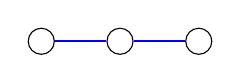
\begin{tikzpicture}
        \node[circle,draw] (v6) at (-1,0) {};
        \node[circle,draw] (v0) at (0,0) {};
        \node[circle,draw] (v1) at (1,0) {};

        \draw[thick,blue] (v6) -- (v0);
        \draw[thick,blue] (v0) -- (v1);
    \end{tikzpicture}
\end{center}

There are some scenarios which didn't happen in the example but need to be handle to make sure our algorithm works in the general case.
There are some special rules for handling vertices that had degree 1 in the original graph which are rather uninterresting.
Refer to the GitHub repository to find them.
Moreover, it can happen that we explore a green edge from both sides at the same time.
Then we will delete that edge to avoid other issues.

\begin{center}
    \begin{tikzpicture}
        % DeleteRule(
        %         name="Propagate update (node already reachable)",
        %         input={"yellow": 1, "lime": 1},
        %         rewiring={},
        %     ),
        \begin{scope}[xshift=-4cm]
            \begin{scope}[xshift=-2cm]
                \node[circle,draw,fill] (A) at (0, 0) {};
                \node[circle,draw] (B) at (-1,0) {};
                \node[circle,draw] (C) at (1,0) {};
                
                \draw[thick,yellow] (A) -- (B);
                \draw[thick,forestgreen] (A) -- (C);
            \end{scope}
        
            \draw [line width=1pt, double distance=3pt, arrows = {-Latex[length=0pt 3 0]}] (-0.5,0) -- node[above] {(29)} (0.5,0);
            
            \begin{scope}[xshift=2.2cm]
                \node[circle,draw] (B) at (-1,0) {};
                \node[circle,draw] (C) at (1,0) {};
            \end{scope}
        \end{scope}
    \end{tikzpicture}
\end{center}

This complete my more complex example of determining the length of the shortest paths between two vertices in a graph.
